% Borrador de revisión en sala — compilar con: tesis/compilar_borrador.sh
\documentclass[12pt,letterpaper,oneside]{report}
\usepackage[letterpaper,margin=2.54cm,headheight=15pt]{geometry}
\usepackage{fontspec}
\usepackage{amsmath,amssymb}
\setmainfont{Liberation Serif}
\setmonofont{DejaVu Sans Mono}[Scale=0.82]
\usepackage{polyglossia}
\setdefaultlanguage{spanish}
\gappto\captionsspanish{\renewcommand{\tablename}{Tabla}\renewcommand{\listtablename}{Índice de Tablas}}
\usepackage{setspace}\onehalfspacing
\usepackage{graphicx,float,booktabs,array,multirow,longtable,tabularx}
\usepackage[table]{xcolor}
\usepackage{siunitx}\sisetup{output-decimal-marker={.},exponent-product=\times}
\usepackage[skip=4pt]{caption}
\captionsetup{labelfont=bf,textfont=it,singlelinecheck=false,justification=raggedright,labelsep=newline}
\usepackage{needspace}
\usepackage{titlesec}
\usepackage{fancyhdr}
\usepackage{enumitem}\setlist{noitemsep,topsep=3pt}
\usepackage{listings}
\usepackage[most]{tcolorbox}
\usepackage{tocloft}
\usepackage[round]{natbib}
\setcitestyle{authoryear,round,aysep={,},yysep={;},notesep={, }}
\usepackage[hidelinks]{hyperref}
\usepackage{xurl}

\definecolor{marino}{HTML}{0B1F4B}
\definecolor{cian}{HTML}{00A3C4}
\definecolor{gris}{HTML}{555555}
\definecolor{fondocod}{HTML}{F5F7FA}

% ===== Variables editables de la carátula y del documento =====
\newcommand{\ProyNum}{38}
\newcommand{\Titulo}{Construcción de una Red Neuronal Artificial desde Cero utilizando Rust}
\newcommand{\Materia}{Programación 1}
\newcommand{\Sigla}{INF120}
\newcommand{\Grupo}{SH-SD}
\newcommand{\DocenteTutor}{MSc. Ing. Víctor Hugo Acosta Ortega}
\newcommand{\CoordinadorIICCT}{MSc. Edwin Vargas Yapura}
\newcommand{\Ciudad}{Santa Cruz de la Sierra -- Bolivia}
\newcommand{\Anio}{2026}
\newcommand{\Evento}{Feria Facultativa de Proyectos de Investigación y Emprendimiento FICCT 2-2026}
\newcommand{\LogoFICCT}{../assets/logos/logo_ficct_escudo.jpeg}
\newcommand{\LogoUAGRM}{../assets/logos/logo_uagrm.jpeg}
\newcommand{\LogoIICCT}{../assets/logos/logo_iicct.jpeg}
\newcommand{\CartaCompromiso}{../assets/docs/carta_compromiso.jpeg}
\newcommand{\Repositorio}{https://github.com/Noxy-bit/Redes-Neuronales-Rust}

% Generado por tesis/scripts/resultados.py desde resultados/*.csv — no editar a mano.
\newcommand{\EunoEpocas}{1000}
\newcommand{\EunoAlpha}{0.01}
\newcommand{\EunoMseIni}{14.883241}
\newcommand{\EunoMseFin}{\num{4.599e-18}}
\newcommand{\EunoPesoIni}{0.836805}
\newcommand{\EunoPesoFin}{1.999999999}
\newcommand{\EunoSesgoFin}{\num{4.834e-9}}
\newcommand{\EunoPredSeis}{11.999999998}
\newcommand{\EdosEpocas}{10000}
\newcommand{\EdosAlpha}{0.5}
\newcommand{\EdosMsePer}{0.251709}
\newcommand{\EdosAccPer}{25.00\,\%}
\newcommand{\EdosMseMul}{\num{1.329e-4}}
\newcommand{\EdosAccMul}{100.00\,\%}
\newcommand{\EdosMseBaja}{0.232847}
\newcommand{\EdosConvBaja}{no alcanzada}
\newcommand{\EdosMseOptima}{0.000133}
\newcommand{\EdosConvOptima}{655}
\newcommand{\EdosMseAlta}{0.500000}
\newcommand{\EdosConvAlta}{no alcanzada}
\newcommand{\EtresEpocas}{1000}
\newcommand{\EtresAlpha}{0.5}
\newcommand{\EtresMseEnt}{\num{1.801e-4}}
\newcommand{\EtresMsePru}{0.010767}
\newcommand{\EtresAccEnt}{100.00\,\%}
\newcommand{\EtresAccPru}{97.60\,\%}
\newcommand{\EtresNEnt}{25}
\newcommand{\EtresNPru}{250}
\newcommand{\PeFilas}{34}
\newcommand{\PeXorEsc}{XOR (2-2-1 sigmoid)}
\newcommand{\BinKiB}{682.6}
\newcommand{\BenchSO}{linux}
\newcommand{\BenchArch}{x86\_64}
\newcommand{\OfCommit}{8667b4c}
\newcommand{\OfRustc}{1.99.1}
\newcommand{\OfBinKiB}{499.7}
\newcommand{\OfPruebas}{0}
\newcommand{\OfClippyErr}{1}
\newcommand{\OfClippyWarn}{27}
\newcommand{\OfWarnBuild}{24}
\newcommand{\OfLinEpocas}{1151}
\newcommand{\OfLinAlpha}{0.02}
\newcommand{\OfLinN}{6}
\newcommand{\OfLinPeso}{1.9999996}
\newcommand{\OfBoolEpocas}{250}
\newcommand{\OfBoolAlpha}{0.5}
\newcommand{\OfBoolW}{6.307747}
\newcommand{\OfBoolB}{-2.94058}
\newcommand{\OfBoolPcero}{0.0502}
\newcommand{\OfBoolPuno}{0.9667}
\newcommand{\OfVocEpocas}{500}
\newcommand{\OfVocAlpha}{0.3}
\newcommand{\OfVocCambioFin}{0.000445}
\newcommand{\OfParedLin}{8.71}
\newcommand{\OfParedBool}{10.03}
\newcommand{\OfParedVoc}{40.10}
\newcommand{\OfCompLin}{1.67}
\newcommand{\OfCompBool}{1.18}
\newcommand{\OfCompVoc}{7.34}
\newcommand{\OfLinMseIni}{95.33}
\newcommand{\OfLinMseFin}{\num{9.470e-13}}
\newcommand{\OfLinBias}{\num{1.9e-6}}
\newcommand{\OfVocConfMin}{98.99\,\%}
\newcommand{\OfVocConfMax}{99.38\,\%}
\newcommand{\OfVocalAProb}{99.32\,\%}
\newcommand{\OfBoolAcc}{100.00\,\%}
\newcommand{\OfVocAcc}{100.00\,\%}
\newcommand{\TablaEuno}{%
0 & 0.836805 & 0.000000 & \num{1.488e1} & 4.184026 \\
1 & 1.681098 & 0.252511 & \num{6.993e-1} & 8.658000 \\
2 & 1.870406 & 0.304295 & \num{4.073e-2} & 9.656326 \\
5 & 1.927720 & 0.303738 & \num{1.800e-2} & 9.942339 \\
10 & 1.934502 & 0.277698 & \num{1.517e-2} & 9.950211 \\
50 & 1.968179 & 0.134918 & \num{3.582e-3} & 9.975811 \\
100 & 1.987093 & 0.054725 & \num{5.893e-4} & 9.990188 \\
250 & 1.999139 & 0.003652 & \num{2.625e-6} & 9.999345 \\
500 & 1.999991 & 0.000040 & \num{3.164e-10} & 9.999993 \\
750 & 2.000000 & 0.000000 & \num{3.815e-14} & 10.000000 \\
1000 & 2.000000 & 0.000000 & \num{4.599e-18} & 10.000000 \\
}
\newcommand{\TablaEdos}{%
$(0,0)$ & 0 & 0.5331 & 0.0058 \\
$(0,1)$ & 1 & 0.5000 & 0.9891 \\
$(1,0)$ & 1 & 0.4669 & 0.9889 \\
$(1,1)$ & 0 & 0.4340 & 0.0161 \\
}
\newcommand{\TablaEdosLr}{%
Baja & 0.01 & 0.232847 & 75.00\,\% & no alcanzada \\
Óptima & 0.5 & 0.000133 & 100.00\,\% & 655 \\
Alta & 50 & 0.500000 & 50.00\,\% & no alcanzada \\
}
\newcommand{\TablaEtresRuido}{%
1 & 50 & 100.00\,\% \\
2 & 50 & 100.00\,\% \\
3 & 50 & 100.00\,\% \\
4 & 50 & 94.00\,\% \\
5 & 50 & 94.00\,\% \\
}
\newcommand{\TablaConfusion}{%
\textbf{A} & 49 & 1 & 0 & 0 & 0 \\
\textbf{E} & 0 & 48 & 1 & 1 & 0 \\
\textbf{I} & 0 & 0 & 50 & 0 & 0 \\
\textbf{O} & 0 & 0 & 0 & 49 & 1 \\
\textbf{U} & 0 & 0 & 0 & 2 & 48 \\
}
\newcommand{\TablaEscritorio}{%
1 & 1 & 2 & 0.8368 & 0.0000 & 0.8368 & -1.1632 & -2.3264 & 0.8601 & 0.0233 \\
2 & 2 & 4 & 0.8601 & 0.0233 & 1.7434 & -2.2566 & -9.0264 & 0.9503 & 0.0684 \\
3 & 3 & 6 & 0.9503 & 0.0684 & 2.9194 & -3.0806 & -18.4836 & 1.1352 & 0.1300 \\
4 & 4 & 8 & 1.1352 & 0.1300 & 4.6707 & -3.3293 & -26.6345 & 1.4015 & 0.1966 \\
5 & 5 & 10 & 1.4015 & 0.1966 & 7.2042 & -2.7958 & -27.9583 & 1.6811 & 0.2525 \\
6 & 1 & 2 & 1.6811 & 0.2525 & 1.9336 & -0.0664 & -0.1328 & 1.6824 & 0.2538 \\
7 & 2 & 4 & 1.6824 & 0.2538 & 3.6187 & -0.3813 & -1.5252 & 1.6977 & 0.2615 \\
8 & 3 & 6 & 1.6977 & 0.2615 & 5.3545 & -0.6455 & -3.8730 & 1.7364 & 0.2744 \\
9 & 4 & 8 & 1.7364 & 0.2744 & 7.2200 & -0.7800 & -6.2399 & 1.7988 & 0.2900 \\
10 & 5 & 10 & 1.7988 & 0.2900 & 9.2840 & -0.7160 & -7.1599 & 1.8704 & 0.3043 \\
}
\newcommand{\TablaBench}{%
y$=$2x & 1-1 & 2 & 100 & 0.150 & 1.504 & 51.0 \\
y$=$2x & 1-1 & 2 & 1000 & 4.879 & 4.879 & 50.0 \\
y$=$2x & 1-1 & 2 & 10000 & 31.644 & 3.164 & 49.6 \\
XOR & 2-4-1 & 17 & 100 & 3.607 & 36.075 & 220.4 \\
XOR & 2-4-1 & 17 & 1000 & 6.037 & 6.037 & 231.0 \\
XOR & 2-4-1 & 17 & 10000 & 51.933 & 5.193 & 221.1 \\
XOR & 2-4-1 & 17 & 100000 & 523.415 & 5.234 & 220.4 \\
vocales & 25-10-5 & 315 & 10 & 0.340 & 34.008 & 430.3 \\
vocales & 25-10-5 & 315 & 100 & 6.590 & 65.897 & 534.7 \\
vocales & 25-10-5 & 315 & 1000 & 59.352 & 59.352 & 531.0 \\
}
\newcommand{\TablaEscritorioXor}{%
1 & (0, 0) & 0 & 1 & 1 & 0.0000 & 0.5000 & -0.0759 & 0.0000 & 0.0380 \\
1 & (0, 0) & 0 & 1 & 2 & 0.0000 & 0.5000 & 0.0605 & 0.0000 & -0.0303 \\
1 & (0, 0) & 0 & 2 & 1 & -0.1326 & 0.4669 & 0.2324 & 0.0000 & -0.1162 \\
2 & (0, 1) & 1 & 1 & 1 & -0.7951 & 0.3111 & 0.0781 & 0.0380 & -0.0011 \\
2 & (0, 1) & 1 & 1 & 2 & -0.4119 & 0.3985 & -0.0630 & -0.0303 & 0.0012 \\
2 & (0, 1) & 1 & 2 & 1 & -0.1489 & 0.4628 & -0.2671 & -0.1162 & 0.0173 \\
}
\newcommand{\TablaHamming}{%
A & 0 & 8 & 15 & 8 & 13 \\
E & 8 & 0 & 7 & 10 & 11 \\
I & 15 & 7 & 0 & 13 & 14 \\
O & 8 & 10 & 13 & 0 & 5 \\
U & 13 & 11 & 14 & 5 & 0 \\
}
\newcommand{\TablaOfLineal}{%
0 & 0.0000000 & 0.0000000 & \num{9.533e1} \\
20 & 1.9509635 & 0.2773890 & \num{2.090e-2} \\
40 & 1.9603254 & 0.2244305 & \num{1.368e-2} \\
60 & 1.9678999 & 0.1815828 & \num{8.957e-3} \\
100 & 1.9789869 & 0.1188666 & \num{3.838e-3} \\
200 & 1.9927145 & 0.0412120 & \num{4.614e-4} \\
400 & 1.9991243 & 0.0049539 & \num{6.666e-6} \\
600 & 1.9998947 & 0.0005955 & \num{9.639e-8} \\
800 & 1.9999872 & 0.0000716 & \num{1.404e-9} \\
1000 & 1.9999985 & 0.0000086 & \num{2.080e-11} \\
1151 & 1.9999996 & 0.0000019 & \num{9.470e-13} \\
}
\newcommand{\TablaOfLinPred}{%
1 & 2.000 & 2.00000 & +0.0000014 \\
2 & 4.000 & 4.00000 & +0.0000010 \\
3 & 6.000 & 6.00000 & +0.0000010 \\
4 & 8.000 & 8.00000 & +0.0000000 \\
7 & 14.000 & 14.00000 & -0.0000010 \\
8 & 16.000 & 16.00000 & -0.0000010 \\
}
\newcommand{\TablaOfBool}{%
1 & -0.250000 & +0.000000 & 0.125000 & 0.000000 & 0.5000 & 0.5312 \\
2 & -0.234395 & +0.015605 & 0.242198 & -0.007802 & 0.4980 & 0.5583 \\
5 & -0.198723 & +0.046151 & 0.556493 & -0.064088 & 0.4840 & 0.6207 \\
10 & -0.162303 & +0.065162 & 0.994605 & -0.213349 & 0.4469 & 0.6860 \\
25 & -0.110873 & +0.058690 & 1.978151 & -0.696539 & 0.3326 & 0.7827 \\
50 & -0.072084 & +0.038044 & 3.081302 & -1.283192 & 0.2170 & 0.8579 \\
100 & -0.040566 & +0.020861 & 4.413019 & -1.976101 & 0.1217 & 0.9196 \\
150 & -0.027706 & +0.014109 & 5.243839 & -2.401078 & 0.0831 & 0.9449 \\
200 & -0.020904 & +0.010594 & 5.842056 & -2.704930 & 0.0627 & 0.9584 \\
250 & -0.016736 & +0.008457 & 6.307747 & -2.940580 & 0.0502 & 0.9667 \\
}
\newcommand{\TablaOfVoc}{%
A & 0.26 & 0.67 & 0.93 & 0.96 & 0.99 & A & 99.32 & 99.32 \\
E & 0.27 & 0.60 & 0.90 & 0.95 & 0.99 & E & 99.07 & 0.36 \\
I & 0.26 & 0.69 & 0.93 & 0.97 & 0.99 & I & 99.38 & 0.01 \\
O & 0.24 & 0.57 & 0.89 & 0.95 & 0.99 & O & 98.99 & 0.30 \\
U & 0.24 & 0.62 & 0.91 & 0.96 & 0.99 & U & 99.17 & 0.01 \\
}
\newcommand{\TablaOfTiempos}{%
$y = 2x$ & \texttt{cargo run -- lineal} & 8.71 & 1.67 \\
Booleano & \texttt{cargo run -- booleano} & 10.03 & 1.18 \\
Vocales & \texttt{cargo run -- vocal} & 40.10 & 7.34 \\
}


% Títulos sobrios y protegidos contra quedar huérfanos
\titleformat{\chapter}[display]{\normalfont\bfseries\color{marino}\centering}{\large CAPÍTULO \thechapter}{4pt}{\LARGE}
\titlespacing*{\chapter}{0pt}{-10pt}{18pt}
\titleformat{\section}{\needspace{6\baselineskip}\normalfont\large\bfseries\color{marino}}{\thesection}{0.6em}{}
\titleformat{\subsection}{\needspace{5\baselineskip}\normalfont\bfseries\itshape}{\thesubsection}{0.6em}{}

\pagestyle{fancy}\fancyhf{}
\fancyhead[L]{\small\color{gris}RN — Redes Neuronales desde Cero en Rust}
\fancyhead[R]{\small\color{gris}Proyecto \#\ProyNum}
\fancyfoot[C]{\thepage}
\renewcommand{\headrulewidth}{0.3pt}
\fancypagestyle{plain}{\fancyhf{}\fancyfoot[C]{\thepage}\renewcommand{\headrulewidth}{0pt}}

\lstdefinelanguage{Rust}{morekeywords={fn,let,mut,pub,struct,enum,impl,trait,for,in,if,else,match,return,use,mod,self,Self,where,const,as,ref,while,loop,break,continue,crate,super,dyn,type},
  sensitive=true,morecomment=[l]{//},morestring=[b]"}
\lstset{language=Rust,basicstyle=\ttfamily\footnotesize\linespread{1}\selectfont,numbers=left,numberstyle=\tiny\color{gris},
  keywordstyle=\color{marino}\bfseries,commentstyle=\color{cian!70!black}\itshape,stringstyle=\color{purple!70!black},
  backgroundcolor=\color{fondocod},frame=single,rulecolor=\color{gray!40},breaklines=true,columns=fullflexible,
  keepspaces=true,showstringspaces=false,xleftmargin=1.5em,framexleftmargin=1.5em,literate={á}{{\'a}}1 {é}{{\'e}}1 {í}{{\'i}}1 {ó}{{\'o}}1 {ú}{{\'u}}1 {ñ}{{\~n}}1 {·}{{$\cdot$}}1 {×}{{$\times$}}1 {α}{{$\alpha$}}1 {δ}{{$\delta$}}1 {⊙}{{$\odot$}}1 {ᵀ}{{$^T$}}1 {≫}{{$\gg$}}1}
\renewcommand{\lstlistingname}{Código}
\renewcommand{\lstlistlistingname}{Lista de Códigos}
\renewcommand{\bibname}{Bibliografía}

\newtcolorbox{nota}[1][Nota técnica]{colback=cian!6,colframe=cian!70!black,fonttitle=\bfseries,title=#1,boxrule=0.6pt,arc=2pt,left=6pt,right=6pt}

% Bibliografía APA 7: sangría francesa de 1.27 cm
\setlength{\bibhang}{1.27cm}\setlength{\bibsep}{6pt}

\setlength{\emergencystretch}{3em}
\begin{document}
\pagenumbering{roman}
% ================= CARÁTULA =================
\begin{titlepage}
\centering
{\large\bfseries UNIVERSIDAD AUTÓNOMA GABRIEL RENÉ MORENO\par}
\vspace{2pt}
{\bfseries FACULTAD DE INGENIERÍA EN CIENCIAS DE LA COMPUTACIÓN\\ Y TELECOMUNICACIONES\par}
\vspace{10pt}
\includegraphics[height=3.6cm]{\LogoFICCT}\par
\vspace{10pt}
{\small \Evento\par}
\vspace{14pt}
{\color{marino}\rule{0.8\textwidth}{0.8pt}\par\vspace{6pt}
\LARGE\bfseries \Titulo\par\vspace{6pt}\rule{0.8\textwidth}{0.8pt}\par}
\vspace{8pt}
{\large Proyecto N.º \ProyNum\par}
\vspace{10pt}
\begin{tabular}{@{}rl@{}}
\textbf{Materia:} & \Materia{} -- \Sigla \\
\textbf{Grupo:} & \Grupo \\
\textbf{Docente tutor:} & \DocenteTutor{} \\
\textbf{Coordinador IICCT:} & \CoordinadorIICCT{} \\
\end{tabular}\par
\vspace{10pt}
{\bfseries Integrantes\par}\vspace{2pt}
{\small
\begin{tabular}{@{}ll@{}}
\toprule
Nombre completo & ORCID \\
\midrule
Ronal Miranda Vasquez & 0009-0003-9735-4920 \\
Oscar Alejandro Nava Orihuela & 0009-0001-0485-3030 \\
Carla Olivia Cano Quispe & 0009-0009-5668-8290 \\
Diana Nayely Diaz Mamani & 0009-0003-0550-4996 \\
Julio Cesar Piuca Achocalla & 0009-0004-0056-5201 \\
\bottomrule
\end{tabular}\par}
\vfill
{\bfseries \Ciudad, \Anio\par}
\end{titlepage}

% ================= IDENTIFICACIÓN DE INVESTIGADORES =================
\setcounter{page}{2}
\chapter*{Identificación de Investigadores y ORCID}
\addcontentsline{toc}{chapter}{Identificación de Investigadores y ORCID}
ORCID (\emph{Open Researcher and Contributor ID}) es un identificador digital persistente, gratuito y único de dieciséis dígitos que distingue a cada investigador de forma inequívoca, aun cuando existan homónimos o variaciones en la escritura de su nombre. Al vincularse con revistas, repositorios y bases de datos, ORCID permite que la producción científica de cada autor sea atribuida correctamente y pueda rastrearse a lo largo de toda su trayectoria académica. Los integrantes del equipo registraron su identificador como parte de la formación en investigación promovida por el Instituto de Investigación de la FICCT (IICCT).

\begin{table}[H]
\caption{Integrantes del equipo de investigación}\label{tab:integrantes}
\small\setlength{\tabcolsep}{4pt}
\begin{tabularx}{\textwidth}{@{}>{\raggedright}X l >{\raggedright}p{2.3cm} l l >{\raggedright\arraybackslash}p{2.4cm}@{}}
\toprule
Nombre completo & Registro & Carrera & Grupo & ORCID & Rol \\
\midrule
Ronal Miranda Vasquez & 226159787 & Ing. Informática & SH-SD & 0009-0003-9735-4920 & Investigador -- Expositor \\
Oscar Alejandro Nava Orihuela & 226037215 & Ing. Informática & SH-SD & 0009-0001-0485-3030 & Investigador -- Expositor \\
Carla Olivia Cano Quispe & 224026879 & Ing. Informática & SH-SD & 0009-0009-5668-8290 & Investigadora -- Expositora \\
Diana Nayely Diaz Mamani & 225028190 & Ing. Sistemas & SH-SD & 0009-0003-0550-4996 & Investigadora -- Expositora \\
Julio Cesar Piuca Achocalla & 224028782 & Ing. Informática & SH-SD & 0009-0004-0056-5201 & Investigador -- Expositor \\
\bottomrule
\end{tabularx}
\par\smallskip{\footnotesize\emph{Nota.} Todos los integrantes pertenecen al grupo SH-SD de la asignatura Programación 1 (INF120). Las áreas de trabajo del equipo se describen en el Anexo~\ref{anx:roles}.}
\end{table}

% ================= AGRADECIMIENTOS =================
\chapter*{Agradecimientos}
\addcontentsline{toc}{chapter}{Agradecimientos}
Al \textbf{\DocenteTutor}, docente de la asignatura Programación 1 (\Sigla), por su guía académica, su exigencia formativa y el respaldo técnico brindado durante el desarrollo de este proyecto.

Al \textbf{\CoordinadorIICCT}, Coordinador del Instituto de Investigación de la FICCT (IICCT) y organizador de la Feria Facultativa FICCT-UAGRM, por el impulso permanente a los semilleros de investigación y por las orientaciones metodológicas que hicieron posible estructurar este trabajo.

A la \textbf{Universidad Autónoma Gabriel René Moreno (UAGRM)}, a la \textbf{Facultad de Ingeniería en Ciencias de la Computación y Telecomunicaciones (FICCT)} y al \textbf{Instituto de Investigación (IICCT)}, por el espacio formativo e institucional que brindan a los estudiantes de los primeros semestres.

A nuestras familias y a cada compañero de equipo, por el esfuerzo colaborativo, la paciencia y el compromiso sostenido durante el desarrollo del proyecto.

% ================= RESUMEN / ABSTRACT =================
\chapter*{Resumen}
\addcontentsline{toc}{chapter}{Resumen}
El presente trabajo documenta la construcción de una red neuronal artificial multicapa implementada desde cero en el lenguaje Rust, utilizando exclusivamente su biblioteca estándar y sin recurrir a \emph{frameworks} de aprendizaje automático ni a bibliotecas externas de álgebra lineal. El proyecto se desarrolló de forma incremental: primero se implementaron vectores y matrices con validación de dimensiones mediante el tipo \texttt{Result}; luego las funciones de activación Sigmoid, ReLU y lineal con sus derivadas analíticas; la función de pérdida de error cuadrático medio (MSE); y finalmente neuronas, capas densas y una red con propagación hacia adelante, retropropagación del error y descenso de gradiente. La corrección del cálculo de gradientes se verificó mediante \emph{gradient checking} numérico dentro de un conjunto de 52 pruebas automatizadas. Se ejecutaron tres experimentos reales y reproducibles (semilla 42): la regresión $y = 2x$ alcanzó un MSE final de \EunoMseFin{}; en la compuerta XOR, el perceptrón de una capa se estancó en una exactitud de \EdosAccPer{} mientras que la red 2-4-1 logró \EdosAccMul{} con MSE de \EdosMseMul{}; y la clasificación de vocales A, E, I, O, U representadas en matrices binarias de $5\times5$ obtuvo \EtresAccPru{} de exactitud sobre \EtresNPru{} muestras de prueba con ruido. Los resultados demuestran que es posible comprender y construir los fundamentos del aprendizaje automático con herramientas abiertas y de bajo costo computacional.

\medskip\noindent\textbf{Palabras clave:} redes neuronales artificiales, retropropagación, descenso de gradiente, Rust, álgebra lineal, aprendizaje automático.

\chapter*{Abstract}
\addcontentsline{toc}{chapter}{Abstract}
This work documents the construction of a multilayer artificial neural network implemented from scratch in the Rust programming language, using only its standard library and without any machine learning frameworks or external linear algebra libraries. The project was developed incrementally: vectors and matrices with dimension checking through the \texttt{Result} type; Sigmoid, ReLU and linear activation functions with analytical derivatives; the mean squared error (MSE) loss; and finally neurons, dense layers and a network with forward propagation, error backpropagation and gradient descent. Gradient correctness was verified through numerical gradient checking within a suite of 52 automated tests. Three real and reproducible experiments were executed (seed 42): the $y = 2x$ regression reached a final MSE of \EunoMseFin{}; on the XOR gate, the single-layer perceptron stalled at \EdosAccPer{} accuracy while the 2-4-1 network reached \EdosAccMul{} with an MSE of \EdosMseMul{}; and the classification of the vowels A, E, I, O, U encoded as $5\times5$ binary matrices achieved \EtresAccPru{} accuracy on \EtresNPru{} noisy test samples. The results show that the foundations of machine learning can be understood and built with open, low-cost tools.

\medskip\noindent\textbf{Keywords:} artificial neural networks, backpropagation, gradient descent, Rust, linear algebra, machine learning.

% ================= ÍNDICES =================
\clearpage
{\singlespacing
\renewcommand{\contentsname}{Índice General}
\tableofcontents
\renewcommand{\listfigurename}{Índice de Figuras}
\clearpage\phantomsection\addcontentsline{toc}{chapter}{Índice de Figuras}
\listoffigures
\renewcommand{\listtablename}{Índice de Tablas}
\clearpage\phantomsection\addcontentsline{toc}{chapter}{Índice de Tablas}
\listoftables
\clearpage\phantomsection\addcontentsline{toc}{chapter}{Lista de Códigos}
\lstlistoflistings
}

\clearpage\pagenumbering{arabic}
\chapter{Contextualización y Antecedentes}\label{cap:contexto}
La inteligencia artificial (IA) ha pasado de ser un campo de investigación especializado a constituir una tecnología transversal presente en la salud, la industria, la educación y los servicios públicos. Este capítulo sitúa el proyecto mediante un enfoque de embudo que recorre cinco niveles de análisis: internacional, nacional, departamental, regional/provincial y local, hasta llegar a la realidad concreta de los estudiantes de Programación 1 de la FICCT.

\section{Nivel internacional}
Las redes neuronales artificiales tienen una historia que se remonta al modelo lógico de neurona de \citet{mcculloch1943} y al perceptrón de \citet{rosenblatt1958}. El entusiasmo inicial se frenó cuando \citet{minsky1969} demostraron formalmente que un perceptrón de una sola capa no puede resolver problemas no linealmente separables como la compuerta XOR. El campo resurgió con la difusión del algoritmo de retropropagación del error \citep{rumelhart1986} y con los resultados teóricos que establecen que una red con al menos una capa oculta es un aproximador universal de funciones continuas \citep{cybenko1989,hornik1989}. Desde la década de 2010, el aprendizaje profundo ha transformado la visión por computador, el procesamiento del lenguaje y numerosos dominios científicos \citep{lecun2015,goodfellow2016}.

El informe \emph{AI Index} de la Universidad de Stanford documenta el crecimiento sostenido de la inversión, las publicaciones y los modelos de IA a escala mundial, así como la concentración de su desarrollo en un número reducido de organizaciones con gran capacidad de cómputo \citep{maslej2024}. En paralelo, la UNESCO ha subrayado la necesidad de formar ciudadanos y profesionales capaces de comprender críticamente los sistemas de IA, y no únicamente de utilizarlos \citep{unesco2022}. Esta tensión revela una brecha formativa: una gran cantidad de usuarios emplea \emph{frameworks} de alto nivel como cajas negras, mientras que comparativamente pocos desarrolladores dominan los fundamentos matemáticos ---álgebra lineal, cálculo diferencial y optimización--- que explican por qué y cómo aprende una red neuronal \citep{deisenroth2020}.

En el ámbito de la ingeniería de sistemas, el lenguaje Rust se ha consolidado como una alternativa que combina el rendimiento de C y C++ con garantías de seguridad de memoria verificadas en tiempo de compilación \citep{matsakis2014,jung2018}. La encuesta anual de desarrolladores de Stack Overflow lo ha ubicado de forma reiterada como el lenguaje más «admirado» por quienes lo utilizan \citep{stackoverflow2024}. Estas características lo vuelven atractivo para la construcción de componentes de alto rendimiento, incluidos los motores numéricos sobre los que se apoya el aprendizaje automático.

\section{Nivel nacional (Bolivia)}
En Bolivia, el marco normativo de las tecnologías de información y comunicación se sustenta en la Ley N.º 164, Ley General de Telecomunicaciones, Tecnologías de Información y Comunicación, que reconoce el acceso a las TIC como un servicio de interés público y promueve el uso de software libre y estándares abiertos en el Estado \citep{bolivia2011}. Este marco favorece iniciativas académicas que, como la presente, se basan en herramientas abiertas y gratuitas.

La transformación digital del país plantea una demanda creciente de profesionales capaces no solo de consumir tecnología, sino de comprenderla y adaptarla a las necesidades locales. En el campo específico de la IA, la formación universitaria todavía tiende a priorizar el uso de herramientas sobre la comprensión de sus fundamentos. Un proyecto que reconstruye una red neuronal desde sus bases matemáticas contribuye a cerrar esa brecha y a formar talento con capacidad de innovación propia.

\begin{nota}[Dato pendiente de verificación]
Para la versión final se recomienda incorporar indicadores nacionales verificables (por ejemplo, estadísticas oficiales de matrícula en carreras de computación o de conectividad) citados en formato APA 7 desde fuentes institucionales. En este borrador no se incluyen cifras que no hayan sido verificadas.
\end{nota}

\section{Nivel departamental (Santa Cruz)}
Santa Cruz es el departamento con mayor dinamismo económico del país y concentra una parte importante de la actividad empresarial y de servicios. Su ecosistema tecnológico incluye empresas de desarrollo de software, emprendimientos digitales y comunidades técnicas que organizan eventos, talleres y encuentros de programación. En este entorno, la demanda de ingenieros con una base matemática y algorítmica sólida es cada vez mayor, porque los productos basados en datos e IA requieren profesionales capaces de diagnosticar, ajustar y optimizar modelos en lugar de limitarse a invocar bibliotecas.

\section{Nivel regional y provincial}
El acceso al conocimiento tecnológico avanzado tiende a concentrarse en las capitales. Para los estudiantes de las provincias del departamento, la dependencia de hardware costoso, de servicios de cómputo en la nube o de licencias pagadas constituye una barrera concreta. El enfoque de este proyecto ---una red neuronal escrita en Rust puro, sin dependencias externas, que se compila en un binario de aproximadamente \BinKiB{}~KiB y entrena los tres experimentos en fracciones de segundo en un computador convencional--- demuestra que es posible estudiar los fundamentos del aprendizaje automático con recursos modestos y materiales de código abierto, lo que favorece la descentralización del conocimiento.

\section{Nivel local (UAGRM -- FICCT)}
En la FICCT, la asignatura Programación 1 (\Sigla) introduce a los estudiantes en el pensamiento algorítmico, las estructuras de control y la modularidad del código. Con frecuencia, los estudiantes de primeros semestres perciben la IA como un tema lejano y reservado a especialistas. Los Semilleros de Investigación impulsados por el IICCT y la Feria Facultativa de Proyectos ofrecen un espacio para acercar estos temas a etapas tempranas de la formación.

Este proyecto aprovecha ese espacio para demostrar que los conceptos de Programación 1 ---funciones, estructuras, ciclos, arreglos y pruebas--- son suficientes para construir, paso a paso, un sistema que aprende a partir de datos. De este modo, el trabajo se convierte en un recurso educativo reutilizable por otros estudiantes de la facultad.

\section{Antecedentes}
Entre los antecedentes conceptuales del proyecto destacan los textos de \citet{haykin2009}, \citet{bishop2006} y \citet{goodfellow2016}, que desarrollan con rigor la teoría de redes neuronales, y el libro abierto de \citet{nielsen2015}, que construye una red neuronal desde cero con fines didácticos. En el ámbito práctico, \citet{lecun1998} sistematizaron recomendaciones para entrenar redes mediante retropropagación, mientras que \citet{glorot2010} y \citet{he2015} propusieron esquemas de inicialización de pesos que hoy son estándar. Respecto a Rust, la documentación oficial \citep{klabnik2023} y el texto de \citet{blandy2021} constituyen las referencias principales sobre el lenguaje y su modelo de propiedad (\emph{ownership}).

\chapter{Planteamiento del Problema y Justificación}\label{cap:problema}
Este capítulo delimita el problema que motiva el proyecto, formula la pregunta de investigación y expone las razones académicas, técnicas y sociales que justifican su desarrollo.

\section{Planteamiento del problema}
El aprendizaje automático suele enseñarse y practicarse mediante \emph{frameworks} de alto nivel que ocultan los detalles de su funcionamiento interno. Con unas pocas líneas de código es posible entrenar un modelo, pero sin comprender cómo se representan los datos en vectores y matrices, cómo se calcula la salida de cada neurona, cómo se mide el error ni cómo se ajustan los pesos. Esta situación genera profesionales que dependen de herramientas cuyo comportamiento no pueden explicar, depurar ni optimizar.

En el contexto local, los estudiantes de los primeros semestres de la FICCT carecen de materiales didácticos que conecten de forma explícita los contenidos de Programación 1 y del álgebra lineal con el funcionamiento real de una red neuronal. Además, buena parte de los recursos disponibles se basa en lenguajes interpretados y bibliotecas externas, lo que dificulta observar el costo computacional real de cada operación.

\subsection{Pregunta de investigación}
¿Es posible construir, con fines educativos y utilizando únicamente la biblioteca estándar del lenguaje Rust, una red neuronal artificial multicapa capaz de aprender relaciones lineales, resolver un problema no lineal como XOR y clasificar patrones visuales simples como las vocales A, E, I, O, U, verificando su correcto funcionamiento mediante pruebas automatizadas y experimentos reproducibles?

\subsection{Delimitación}
\begin{itemize}
\item \textbf{Alcance temático:} redes neuronales densas (\emph{feedforward}) con funciones de activación Sigmoid, ReLU y lineal, pérdida MSE y descenso de gradiente estocástico.
\item \textbf{Alcance técnico:} implementación en Rust (edición 2024) sin crates externos; ejecución en un computador personal convencional.
\item \textbf{Alcance experimental:} tres experimentos progresivos ($y=2x$, XOR y vocales) con datos sintéticos definidos explícitamente en el código.
\item \textbf{Fuera de alcance:} redes convolucionales o recurrentes, aceleración por GPU y conjuntos de datos masivos.
\end{itemize}

\section{Justificación}
\subsection{Justificación académica}
Construir una red neuronal desde cero obliga a traducir cada ecuación matemática en código verificable. Ese ejercicio consolida conocimientos de álgebra lineal (productos matriz-vector, transpuestas, producto de Hadamard), de cálculo diferencial (regla de la cadena) y de programación estructurada, y permite comprender por qué funcionan técnicas que en los \emph{frameworks} aparecen como una sola llamada a función \citep{nielsen2015,deisenroth2020}.

\subsection{Justificación técnica}
Rust ofrece rendimiento comparable al de C sin recolector de basura y con seguridad de memoria garantizada por el compilador \citep{klabnik2023,jung2018}. Su sistema de tipos y el manejo explícito de errores mediante \texttt{Result} permiten detectar en tiempo de ejecución, de forma controlada, errores de dimensión que en otros lenguajes producirían resultados incorrectos silenciosos. Además, su herramienta \texttt{cargo} integra compilación, pruebas y documentación, lo que facilita una metodología de desarrollo verificable.

\subsection{Justificación social y educativa}
El proyecto se publica como código abierto y no requiere hardware especializado, licencias ni conexión permanente a servicios en la nube. Esto lo vuelve accesible para estudiantes de cualquier provincia y lo convierte en un material reutilizable para la enseñanza de la IA en la universidad pública.

\subsection{Viabilidad}
El proyecto es viable porque utiliza herramientas gratuitas (Rust, Cargo, Git, \LaTeX), se ejecuta en equipos convencionales y se apoya en una bibliografía consolidada. La validación mediante pruebas automatizadas y experimentos reproducibles con semilla fija garantiza que los resultados puedan ser verificados por cualquier evaluador.

\chapter{Objetivo General}\label{cap:objgeneral}
El objetivo general orienta la totalidad del proyecto y define el resultado verificable que se espera alcanzar.

\begin{nota}[Objetivo general]
Desarrollar una red neuronal artificial multicapa desde cero utilizando el lenguaje Rust y únicamente su biblioteca estándar, implementando sus fundamentos matemáticos (álgebra lineal, funciones de activación, función de pérdida, retropropagación y descenso de gradiente) y validando su funcionamiento mediante pruebas unitarias y tres experimentos reproducibles de complejidad progresiva.
\end{nota}

\chapter{Objetivos Específicos}\label{cap:objespecificos}
Los objetivos específicos descomponen el objetivo general en metas concretas y medibles, alineadas con las fases de desarrollo del proyecto.

\begin{enumerate}[label=\textbf{OE\arabic*.},leftmargin=3.2em,itemsep=4pt]
\item Implementar estructuras de vectores y matrices con operaciones de suma, resta, producto punto, multiplicación matricial, producto de Hadamard, escalamiento y transpuesta, con validación de dimensiones mediante el tipo \texttt{Result}.
\item Implementar las funciones de activación Sigmoid, ReLU y lineal con sus derivadas analíticas, y la función de pérdida de error cuadrático medio (MSE) con su gradiente.
\item Construir neuronas, capas densas y una red multicapa con inicialización reproducible mediante un generador pseudoaleatorio propio, propagación hacia adelante, retropropagación del error y entrenamiento por descenso de gradiente.
\item Verificar la corrección de la implementación mediante pruebas unitarias en cada módulo, incluida la comparación entre gradientes analíticos y numéricos (\emph{gradient checking}).
\item Ejecutar y analizar tres experimentos progresivos ---regresión $y=2x$, compuerta XOR y clasificación de vocales A, E, I, O, U--- exportando métricas reales (pérdida, exactitud y matriz de confusión) a archivos CSV.
\item Medir el rendimiento real del motor (tiempos de entrenamiento e inferencia y tamaño del binario) compilado en modo \emph{release}.
\end{enumerate}

\chapter{Marco Teórico}\label{cap:marco}
El marco teórico reúne los fundamentos matemáticos que sustentan el funcionamiento de una red neuronal artificial y los fundamentos técnicos del lenguaje Rust que justifican su elección. Cada ecuación de este capítulo tiene una implementación directa en el código fuente del proyecto.

\section{Fundamentos de álgebra lineal}
\subsection{Vectores y matrices}
Un vector $\mathbf{x}\in\mathbb{R}^{n}$ es una lista ordenada de $n$ números reales, interpretada en este trabajo como vector columna. Una matriz $\mathbf{W}\in\mathbb{R}^{m\times n}$ es un arreglo rectangular de $m$ filas y $n$ columnas \citep{strang2016}. En la implementación, las matrices se almacenan en un único arreglo contiguo en orden por filas (\emph{row-major}), de modo que el elemento $w_{ij}$ ocupa la posición $i\cdot n + j$.

\subsection{Operaciones fundamentales}
Sean $\mathbf{x},\mathbf{y}\in\mathbb{R}^{n}$ y $\mathbf{A}\in\mathbb{R}^{m\times k}$, $\mathbf{B}\in\mathbb{R}^{k\times n}$. Las operaciones implementadas son:
\begin{align}
\mathbf{x}\cdot\mathbf{y} &= \sum_{i=1}^{n} x_i y_i, &&\text{(producto punto, } O(n)\text{)}\label{eq:dot}\\
(\mathbf{A}\mathbf{B})_{ij} &= \sum_{l=1}^{k} a_{il}\, b_{lj}, &&\text{(producto matricial, } O(mkn)\text{)}\label{eq:matmul}\\
(\mathbf{x}\odot\mathbf{y})_i &= x_i\, y_i, &&\text{(producto de Hadamard, } O(n)\text{)}\label{eq:hadamard}\\
(\mathbf{A}^{\top})_{ij} &= a_{ji}, &&\text{(transpuesta, } O(mk)\text{)}\label{eq:transpuesta}\\
(\mathbf{x}\,\mathbf{y}^{\top})_{ij} &= x_i\, y_j. &&\text{(producto exterior, } O(n^2)\text{)}\label{eq:outer}
\end{align}
Estas operaciones solo están definidas cuando las dimensiones son compatibles; por ejemplo, el producto $\mathbf{A}\mathbf{B}$ exige que el número de columnas de $\mathbf{A}$ coincida con el número de filas de $\mathbf{B}$. En el proyecto, toda violación de dimensiones produce un error explícito en lugar de un resultado incorrecto.

\section{La neurona artificial}
La neurona artificial, inspirada en el modelo de \citet{mcculloch1943} y en el perceptrón de \citet{rosenblatt1958}, recibe un vector de entradas $\mathbf{x}\in\mathbb{R}^{n}$, lo combina linealmente con un vector de pesos $\mathbf{w}\in\mathbb{R}^{n}$ y un sesgo $b\in\mathbb{R}$, y aplica una función de activación $f$:
\begin{equation}
z = \mathbf{w}\cdot\mathbf{x} + b = \sum_{i=1}^{n} w_i x_i + b, \qquad a = f(z).\label{eq:neurona}
\end{equation}
La suma ponderada $z$ define un hiperplano en el espacio de entradas. Por ello, una única neurona solo puede separar clases que sean linealmente separables, limitación que \citet{minsky1969} formalizaron con el ejemplo de la compuerta XOR.

\section{Funciones de activación}
Las funciones de activación introducen no linealidad; sin ellas, la composición de varias capas seguiría siendo una transformación lineal \citep{goodfellow2016}.

\subsection{Función Sigmoid}
\begin{equation}
\sigma(z) = \frac{1}{1+e^{-z}}, \qquad \sigma'(z) = \sigma(z)\,\bigl(1-\sigma(z)\bigr).\label{eq:sigmoid}
\end{equation}
La derivada se obtiene aplicando la regla del cociente: $\sigma'(z) = \frac{e^{-z}}{(1+e^{-z})^2} = \frac{1}{1+e^{-z}}\cdot\frac{e^{-z}}{1+e^{-z}} = \sigma(z)(1-\sigma(z))$. Su valor máximo es $0.25$ en $z=0$, lo que explica la lentitud del aprendizaje cuando las neuronas se saturan \citep{lecun1998}. Para evitar desbordamientos numéricos, la implementación usa la forma equivalente $\sigma(z) = e^{z}/(1+e^{z})$ cuando $z<0$.

\subsection{Función ReLU}
\begin{equation}
\mathrm{ReLU}(z) = \max(0, z), \qquad \mathrm{ReLU}'(z) = \begin{cases}1 & z>0\\ 0 & z\le 0\end{cases}\label{eq:relu}
\end{equation}
ReLU es computacionalmente económica y mitiga el desvanecimiento del gradiente en redes profundas \citep{glorot2010,he2015}. En $z=0$ la derivada no existe; por convención se adopta el valor $0$.

\subsection{Función lineal}
Para problemas de regresión se utiliza la identidad $f(z)=z$, cuya derivada es $f'(z)=1$.

\section{Función de pérdida: error cuadrático medio}
Dado un vector de predicciones $\hat{\mathbf{y}}\in\mathbb{R}^{n}$ y un vector objetivo $\mathbf{y}\in\mathbb{R}^{n}$, el error cuadrático medio y su gradiente son:
\begin{equation}
\mathcal{L}(\hat{\mathbf{y}},\mathbf{y}) = \frac{1}{n}\sum_{i=1}^{n}(\hat{y}_i - y_i)^2, \qquad \frac{\partial\mathcal{L}}{\partial \hat{y}_i} = \frac{2}{n}(\hat{y}_i - y_i).\label{eq:mse}
\end{equation}
El MSE es siempre no negativo y vale cero únicamente cuando la predicción coincide exactamente con el objetivo \citep{bishop2006}.

\section{Red neuronal multicapa}
Una red multicapa (\emph{multilayer perceptron}) organiza las neuronas en $L$ capas densas. Para la capa $l$ con $n_{l-1}$ entradas y $n_l$ neuronas, los parámetros son la matriz $\mathbf{W}^{(l)}\in\mathbb{R}^{n_l\times n_{l-1}}$ y el vector $\mathbf{b}^{(l)}\in\mathbb{R}^{n_l}$. La propagación hacia adelante es:
\begin{equation}
\mathbf{z}^{(l)} = \mathbf{W}^{(l)}\mathbf{a}^{(l-1)} + \mathbf{b}^{(l)}, \qquad \mathbf{a}^{(l)} = f^{(l)}\bigl(\mathbf{z}^{(l)}\bigr), \qquad \mathbf{a}^{(0)} = \mathbf{x}.\label{eq:forward}
\end{equation}
El teorema de aproximación universal garantiza que una red con una sola capa oculta y un número suficiente de neuronas con activación sigmoidal puede aproximar cualquier función continua en un dominio compacto con precisión arbitraria \citep{cybenko1989,hornik1989}.

\section{Retropropagación del error}
La retropropagación (\emph{backpropagation}) calcula eficientemente el gradiente de la pérdida respecto a todos los parámetros aplicando la regla de la cadena desde la salida hacia la entrada \citep{rumelhart1986}. Se define el error local de la capa $l$ como $\boldsymbol{\delta}^{(l)} = \partial\mathcal{L}/\partial\mathbf{z}^{(l)}$.

\subsection{Derivación paso a paso}
Para la capa de salida $L$, por la regla de la cadena:
\begin{equation}
\delta_j^{(L)} = \frac{\partial\mathcal{L}}{\partial a_j^{(L)}}\cdot\frac{\partial a_j^{(L)}}{\partial z_j^{(L)}} = \frac{2}{n_L}\bigl(a_j^{(L)}-y_j\bigr)\, f'\bigl(z_j^{(L)}\bigr)
\;\Longrightarrow\; \boldsymbol{\delta}^{(L)} = \nabla_{\mathbf{a}}\mathcal{L}\odot f'\bigl(\mathbf{z}^{(L)}\bigr).\label{eq:deltaL}
\end{equation}
Para una capa oculta $l$, cada $z_j^{(l)}$ influye en la pérdida a través de todas las neuronas $k$ de la capa siguiente:
\begin{equation}
\begin{split}
\delta_j^{(l)} &= \sum_{k}\frac{\partial\mathcal{L}}{\partial z_k^{(l+1)}}\frac{\partial z_k^{(l+1)}}{\partial a_j^{(l)}}\frac{\partial a_j^{(l)}}{\partial z_j^{(l)}} = \Bigl(\sum_k w_{kj}^{(l+1)}\delta_k^{(l+1)}\Bigr) f'\bigl(z_j^{(l)}\bigr)\\
\Longrightarrow\quad \boldsymbol{\delta}^{(l)} &= \bigl(\mathbf{W}^{(l+1)\top}\boldsymbol{\delta}^{(l+1)}\bigr)\odot f'\bigl(\mathbf{z}^{(l)}\bigr).
\end{split}\label{eq:deltal}
\end{equation}
Como $z_j^{(l)} = \sum_i w_{ji}^{(l)}a_i^{(l-1)} + b_j^{(l)}$, los gradientes de los parámetros resultan:
\begin{equation}
\frac{\partial\mathcal{L}}{\partial\mathbf{W}^{(l)}} = \boldsymbol{\delta}^{(l)}\,\mathbf{a}^{(l-1)\top}, \qquad \frac{\partial\mathcal{L}}{\partial\mathbf{b}^{(l)}} = \boldsymbol{\delta}^{(l)}.\label{eq:gradW}
\end{equation}
El costo de la retropropagación es del mismo orden que el de la propagación hacia adelante, $O(P)$, donde $P$ es el número total de parámetros, lo que la hace mucho más eficiente que estimar cada derivada por separado \citep{baydin2018}.

\section{Descenso de gradiente}
El descenso de gradiente actualiza cada parámetro en dirección opuesta al gradiente, con una tasa de aprendizaje $\alpha>0$:
\begin{equation}
\mathbf{W}^{(l)} \leftarrow \mathbf{W}^{(l)} - \alpha\,\frac{\partial\mathcal{L}}{\partial\mathbf{W}^{(l)}}, \qquad \mathbf{b}^{(l)} \leftarrow \mathbf{b}^{(l)} - \alpha\,\frac{\partial\mathcal{L}}{\partial\mathbf{b}^{(l)}}.\label{eq:gd}
\end{equation}
En la variante estocástica (SGD) utilizada en este proyecto, la actualización se realiza después de cada muestra \citep{bottou2010}. Una tasa $\alpha$ muy pequeña produce un aprendizaje extremadamente lento; una tasa excesiva provoca oscilaciones, divergencia o saturación de las neuronas \citep{ruder2016}. Este comportamiento se verifica experimentalmente en la Sección~\ref{sec:exp2}.

\section{Inicialización de pesos}
Si todos los pesos se inicializan con el mismo valor, las neuronas de una capa reciben gradientes idénticos y nunca se diferencian. Por ello se emplea inicialización aleatoria uniforme en $[-\ell,\ell]$ con la regla de \citet{glorot2010} para Sigmoid y lineal, y la de \citet{he2015} para ReLU:
\begin{equation}
\ell_{\text{Xavier}} = \sqrt{\frac{6}{n_{\text{in}}+n_{\text{out}}}}, \qquad \ell_{\text{He}} = \sqrt{\frac{6}{n_{\text{in}}}}.\label{eq:init}
\end{equation}

\section{Verificación numérica de gradientes}
Para comprobar que las derivadas analíticas están correctamente implementadas se compara cada componente del gradiente con su aproximación por diferencias centrales \citep{lecun1998,goodfellow2016}:
\begin{equation}
\frac{\partial\mathcal{L}}{\partial\theta} \approx \frac{\mathcal{L}(\theta+\varepsilon)-\mathcal{L}(\theta-\varepsilon)}{2\varepsilon}, \qquad \text{error relativo} = \frac{|g_{\text{num}}-g_{\text{ana}}|}{\max(|g_{\text{num}}|+|g_{\text{ana}}|,\,10^{-12})}.\label{eq:gradcheck}
\end{equation}
El error de truncamiento de esta aproximación es $O(\varepsilon^{2})$, por lo que un error relativo muy pequeño indica que la retropropagación es correcta.

\section{Métricas de evaluación}
Para clasificación se utiliza la exactitud (\emph{accuracy}), definida como la proporción de muestras correctamente clasificadas, y la matriz de confusión $\mathbf{C}\in\mathbb{N}^{K\times K}$, cuyo elemento $c_{ij}$ cuenta las muestras de clase real $i$ predichas como clase $j$. En clasificación multiclase con codificación \emph{one-hot}, la clase predicha es $\hat{k} = \arg\max_k \hat{y}_k$ \citep{bishop2006}.

\section{Fundamentos técnicos de Rust}
Rust es un lenguaje de programación de sistemas compilado, con tipado estático y fuerte, diseñado para ofrecer seguridad de memoria sin recolector de basura \citep{klabnik2023,matsakis2014}.

\subsection{Propiedad, préstamos y tiempos de vida}
El modelo de propiedad (\emph{ownership}) establece que cada valor tiene un único dueño y se libera automáticamente cuando su dueño sale de ámbito. Los préstamos (\emph{borrowing}) permiten referencias inmutables múltiples (\texttt{\&T}) o una única referencia mutable (\texttt{\&mut T}), lo que elimina en tiempo de compilación las carreras de datos y los accesos a memoria liberada \citep{blandy2021}. \citet{jung2018} demostraron formalmente la solidez de estas garantías en el proyecto RustBelt.

\subsection{Manejo explícito de errores}
Rust no utiliza excepciones. Las operaciones que pueden fallar devuelven \texttt{Result<T, E>}, que obliga al programador a tratar el error explícitamente. El operador \texttt{?} propaga el error al llamador de forma concisa. En este proyecto, toda operación de álgebra lineal devuelve \texttt{Result} con un tipo \texttt{MathError} que describe la operación y las dimensiones incompatibles.

\subsection{Traits y abstracciones de costo cero}
Los \emph{traits} definen comportamiento compartido, similar a las interfaces de otros lenguajes. El proyecto define los traits \texttt{ActivationFn} y \texttt{LossFn}, lo que permite añadir nuevas funciones sin modificar la red. Gracias a la monomorfización, estas abstracciones no tienen costo en tiempo de ejecución.

\subsection{Cargo y pruebas integradas}
Cargo es el gestor de paquetes y sistema de compilación de Rust. Permite compilar en modo depuración o optimizado (\texttt{--release}), ejecutar pruebas unitarias con \texttt{cargo test}, analizar el código con \texttt{cargo clippy} y generar documentación a partir de los comentarios \texttt{///} \citep{klabnik2023}.

\chapter{Desarrollo de la Propuesta Solución}\label{cap:propuesta}
Este capítulo describe la arquitectura implementada, la metodología de desarrollo por fases, la estrategia de verificación y los resultados reales obtenidos al ejecutar el binario compilado. Todas las cifras provienen de los archivos \texttt{resultados/*.csv} generados por el comando \texttt{cargo run --release -- --all} con semilla 42.

\section{Metodología de desarrollo}
El proyecto siguió una metodología incremental de seis fases, en la que cada módulo debía superar sus pruebas unitarias antes de iniciar la fase siguiente:
\begin{enumerate}
\item \textbf{Álgebra lineal:} vectores, matrices y errores de dimensión.
\item \textbf{Neurona y activaciones:} Sigmoid, ReLU, lineal y sus derivadas.
\item \textbf{Pérdida:} error cuadrático medio y su gradiente.
\item \textbf{Capa y red:} propagación hacia adelante y retropropagación.
\item \textbf{Aprendizaje:} descenso de gradiente y verificación numérica de gradientes.
\item \textbf{Experimentación:} $y=2x$, XOR, vocales, prueba de escritorio y benchmarks.
\end{enumerate}

\section{Arquitectura del sistema}
El código se organiza como una biblioteca (\texttt{src/lib.rs}) y un binario de línea de comandos (\texttt{src/main.rs}). La biblioteca se divide en tres módulos con responsabilidades separadas (Tabla~\ref{tab:arquitectura}).

\begin{table}[H]
\caption{Módulos de la arquitectura implementada}\label{tab:arquitectura}
\small
\begin{tabularx}{\textwidth}{@{}l >{\raggedright\arraybackslash}X@{}}
\toprule
Archivo & Responsabilidad \\
\midrule
\texttt{math/vector.rs} & Vector $\mathbb{R}^n$: suma, resta, producto punto, Hadamard, escalamiento, norma, \texttt{argmax}. \\
\texttt{math/matrix.rs} & Matriz $\mathbb{R}^{m\times n}$ \emph{row-major}: producto matricial, matriz-vector, transpuesta, producto exterior. \\
\texttt{math/error.rs} & Tipo \texttt{MathError} para dimensiones incompatibles e índices fuera de rango. \\
\texttt{math/rng.rs} & Generador pseudoaleatorio SplitMix64 reproducible (sin crates externos). \\
\texttt{nn/activation.rs} & Trait \texttt{ActivationFn}; Sigmoid, ReLU y lineal con derivadas analíticas. \\
\texttt{nn/loss.rs} & Trait \texttt{LossFn}; MSE y su gradiente. \\
\texttt{nn/neuron.rs} & Neurona individual: pesos, sesgo, suma ponderada y activación. \\
\texttt{nn/layer.rs} & Capa densa: \texttt{forward}, \texttt{backward}, gradientes y actualización. \\
\texttt{nn/network.rs} & Red multicapa: \texttt{forward}, \texttt{backward}, \texttt{predict}, \texttt{train}, evaluación. \\
\texttt{experiments/} & Tres experimentos, prueba de escritorio, benchmarks y escritura de CSV. \\
\texttt{main.rs} & CLI reproducible: \texttt{--all}, \texttt{--exp1..3}, \texttt{--bench}, \texttt{--export}, \texttt{--seed}. \\
\bottomrule
\end{tabularx}
\par\smallskip{\footnotesize\emph{Nota.} El archivo \texttt{Cargo.toml} no declara ninguna dependencia: todo el sistema utiliza exclusivamente la biblioteca estándar de Rust.}
\end{table}

\subsection{Flujo de datos}
El flujo de una iteración de entrenamiento es: (1) la entrada $\mathbf{x}$ atraviesa cada capa calculando $\mathbf{z}^{(l)}$ y $\mathbf{a}^{(l)}$, que se almacenan en caché; (2) se calcula la pérdida MSE y su gradiente respecto a la salida; (3) cada capa, de la última a la primera, calcula $\boldsymbol{\delta}^{(l)}$, sus gradientes y el gradiente que transmite a la capa anterior; (4) todos los parámetros se actualizan con la Ecuación~\eqref{eq:gd}. El Código~\ref{cod:train} muestra que este flujo se expresa en Rust de forma casi literal.

\lstinputlisting[caption={Iteración de entrenamiento (\texttt{src/nn/network.rs})},label=cod:train]{generado/codigo/train_step.rs}

\subsection{Implementación de la retropropagación}
El Código~\ref{cod:backward} implementa las Ecuaciones~\eqref{eq:deltaL}--\eqref{eq:gradW}: el producto de Hadamard entre el gradiente recibido y la derivada de la activación produce $\boldsymbol{\delta}$; el producto exterior $\boldsymbol{\delta}\,\mathbf{x}^{\top}$ produce el gradiente de los pesos; y $\mathbf{W}^{\top}\boldsymbol{\delta}$ produce el gradiente que se transmite a la capa anterior.

\lstinputlisting[caption={Retropropagación en una capa densa (\texttt{src/nn/layer.rs})},label=cod:backward]{generado/codigo/layer_backward.rs}

\subsection{Manejo de errores de dimensión}
El Código~\ref{cod:matmul} muestra el producto matricial: antes de operar, se verifica que las dimensiones sean compatibles y, en caso contrario, se devuelve un \texttt{MathError::DimensionMismatch} que indica la operación y las formas involucradas.

\lstinputlisting[caption={Producto matricial con validación de dimensiones (\texttt{src/math/matrix.rs})},label=cod:matmul]{generado/codigo/matmul.rs}

\subsection{Reproducibilidad}
Para que cualquier evaluador obtenga exactamente los mismos resultados, los pesos iniciales y el ruido de los datos se generan con un PRNG SplitMix64 propio con semilla fija (por defecto 42), modificable mediante \texttt{--seed}.

\lstinputlisting[caption={Generador pseudoaleatorio SplitMix64 (\texttt{src/math/rng.rs})},label=cod:rng]{generado/codigo/rng.rs}

\section{Estrategia de verificación}
La suite de pruebas cuenta con 52 pruebas automatizadas (51 en la biblioteca y 1 en la CLI), todas aprobadas. Incluyen valores calculados a mano, errores de dimensión, propiedades matemáticas (por ejemplo, $(\mathbf{A}^{\top})^{\top}=\mathbf{A}$), determinismo del PRNG, convergencia real de $y=2x$ y XOR, y verificación numérica de gradientes según la Ecuación~\eqref{eq:gradcheck} sobre redes 2-4-1, 3-5-4-2 y 25-10-5. El detalle se presenta en el Anexo~\ref{anx:tests}. Adicionalmente, \texttt{cargo clippy --all-targets} no reporta advertencias.

\section{Prueba de escritorio}
La prueba de escritorio registra cada operación de las primeras iteraciones del entrenamiento. Para la neurona lineal de $y=2x$ ($\alpha = 0.01$), la primera iteración con $x=1$, $y=2$ y peso inicial $w_0 = 0.836805$, $b_0 = 0$ es:
\begin{align*}
z &= w_0 x + b_0 = 0.836805\cdot 1 + 0 = 0.836805, & a &= z = 0.836805,\\
e &= a - y = -1.163195, & \mathcal{L} &= e^2 = 1.353022,\\
\delta &= 2e\cdot f'(z) = -2.326389, & \partial\mathcal{L}/\partial w &= \delta\, x = -2.326389,\\
w_1 &= w_0 - \alpha\,\delta x = 0.860069, & b_1 &= b_0 - \alpha\,\delta = 0.023264.
\end{align*}
La Tabla~\ref{tab:escritorio} resume las diez primeras iteraciones (dos épocas). La traza completa, que también incluye las primeras iteraciones de la red XOR 2-2-1, contiene \PeFilas{} filas y se encuentra en el archivo \path{resultados/prueba_escritorio.csv}.

\begin{table}[H]
\caption{Prueba de escritorio de la neurona lineal para $y=2x$ (primeras 10 iteraciones)}\label{tab:escritorio}
\footnotesize\setlength{\tabcolsep}{3.5pt}
\begin{tabular}{@{}rrrrrrrrrr@{}}
\toprule
It. & $x$ & $y$ & $w$ & $b$ & $z$ & $e$ & $\partial\mathcal{L}/\partial w$ & $w'$ & $b'$ \\
\midrule
\TablaEscritorio
\bottomrule
\end{tabular}
\par\smallskip{\footnotesize\emph{Nota.} $e = \hat{y}-y$; $w'$ y $b'$ son los parámetros después de la actualización. Fuente: \texttt{resultados/prueba\_escritorio.csv}.}
\end{table}

\section{Experimento 1: regresión lineal $y=2x$}\label{sec:exp1}
\subsection{Diseño}
Se entrena una neurona con activación lineal (red 1-1, dos parámetros) sobre los pares $(1,2),(2,4),(3,6),(4,8),(5,10)$ durante \EunoEpocas{} épocas con $\alpha=\EunoAlpha$. La solución exacta es $w=2$, $b=0$.

\subsection{Resultados}
El MSE descendió desde \EunoMseIni{} en la época 0 hasta \EunoMseFin{} en la época \EunoEpocas. Los parámetros finales fueron $w=\EunoPesoFin$ y $b=\EunoSesgoFin$, y la predicción para el valor no visto $x=6$ fue $\hat{y}=\EunoPredSeis$ (Tabla~\ref{tab:exp1} y Figura~\ref{fig:exp1}).

\begin{table}[H]
\caption{Evolución del entrenamiento del Experimento 1}\label{tab:exp1}
\small
\begin{tabular}{@{}rrrrr@{}}
\toprule
Época & Peso $w$ & Sesgo $b$ & MSE & $\hat{y}(x=5)$ \\
\midrule
\TablaEuno
\bottomrule
\end{tabular}
\par\smallskip{\footnotesize\emph{Nota.} Fuente: \texttt{resultados/exp1\_y2x.csv}.}
\end{table}

\begin{figure}[H]
\caption{Pérdida y parámetros durante el entrenamiento de $y=2x$}\label{fig:exp1}
\centering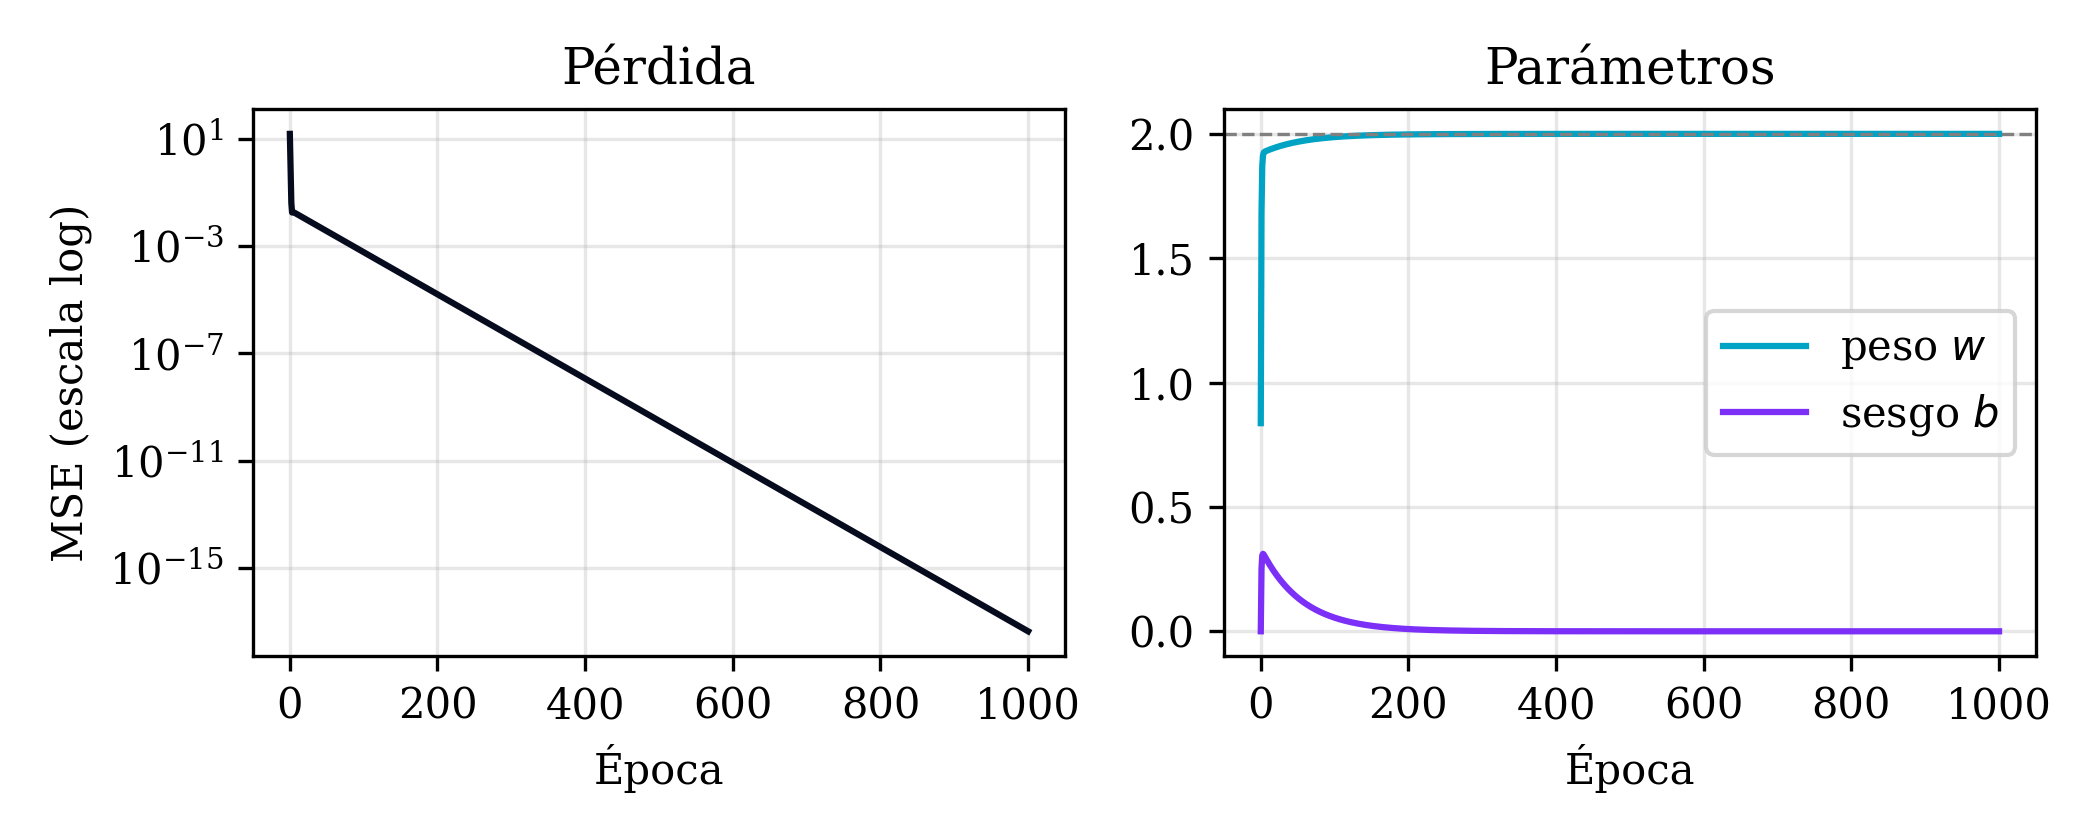
\includegraphics[width=\textwidth]{figuras/exp1_y2x.png}
\par\smallskip{\footnotesize\raggedright\emph{Nota.} Izquierda: MSE en escala logarítmica. Derecha: el peso converge a 2 (línea discontinua) y el sesgo a 0.\par}
\end{figure}

\subsection{Análisis}
La pérdida decrece de forma monótona y casi exponencial, comportamiento esperado para un problema convexo con una tasa de aprendizaje adecuada. El MSE final, del orden de $10^{-18}$, está en el límite de la precisión de la aritmética de punto flotante de doble precisión. La neurona generaliza correctamente fuera del rango de entrenamiento.

\section{Experimento 2: compuerta XOR}\label{sec:exp2}
\subsection{Diseño}
La función XOR devuelve 1 cuando sus dos entradas binarias son distintas. Se comparan un perceptrón de una capa (2-1, Sigmoid) y una red multicapa 2-4-1 (Sigmoid/Sigmoid), ambos entrenados durante \EdosEpocas{} épocas con $\alpha=\EdosAlpha$. Además, la red 2-4-1 se entrena con tres tasas: baja ($0.01$), óptima ($0.5$) y alta ($50$).

\subsection{Resultados}
El perceptrón terminó con MSE de \EdosMsePer{} y exactitud de \EdosAccPer, mientras que la red multicapa alcanzó MSE de \EdosMseMul{} y exactitud de \EdosAccMul{} (Tabla~\ref{tab:exp2}).

\begin{table}[H]
\caption{Predicciones finales para XOR}\label{tab:exp2}
\small
\begin{tabular}{@{}lrrr@{}}
\toprule
Entrada & Objetivo & Perceptrón 2-1 & Multicapa 2-4-1 \\
\midrule
\TablaEdos
\bottomrule
\end{tabular}
\par\smallskip{\footnotesize\emph{Nota.} Se clasifica como 1 cuando la salida es $\ge 0.5$. Fuente: \texttt{resultados/exp2\_xor.csv}.}
\end{table}

\begin{table}[H]
\caption{Efecto de la tasa de aprendizaje en la red 2-4-1 para XOR}\label{tab:exp2lr}
\small
\begin{tabular}{@{}lrrrl@{}}
\toprule
Escenario & $\alpha$ & MSE final & Exactitud & Época de convergencia \\
\midrule
\TablaEdosLr
\bottomrule
\end{tabular}
\par\smallskip{\footnotesize\emph{Nota.} Convergencia: primera época con MSE $<0.01$. Fuente: \texttt{resultados/exp2\_xor\_lr.csv}.}
\end{table}

\begin{figure}[H]
\caption{Curvas de pérdida del Experimento 2}\label{fig:exp2}
\centering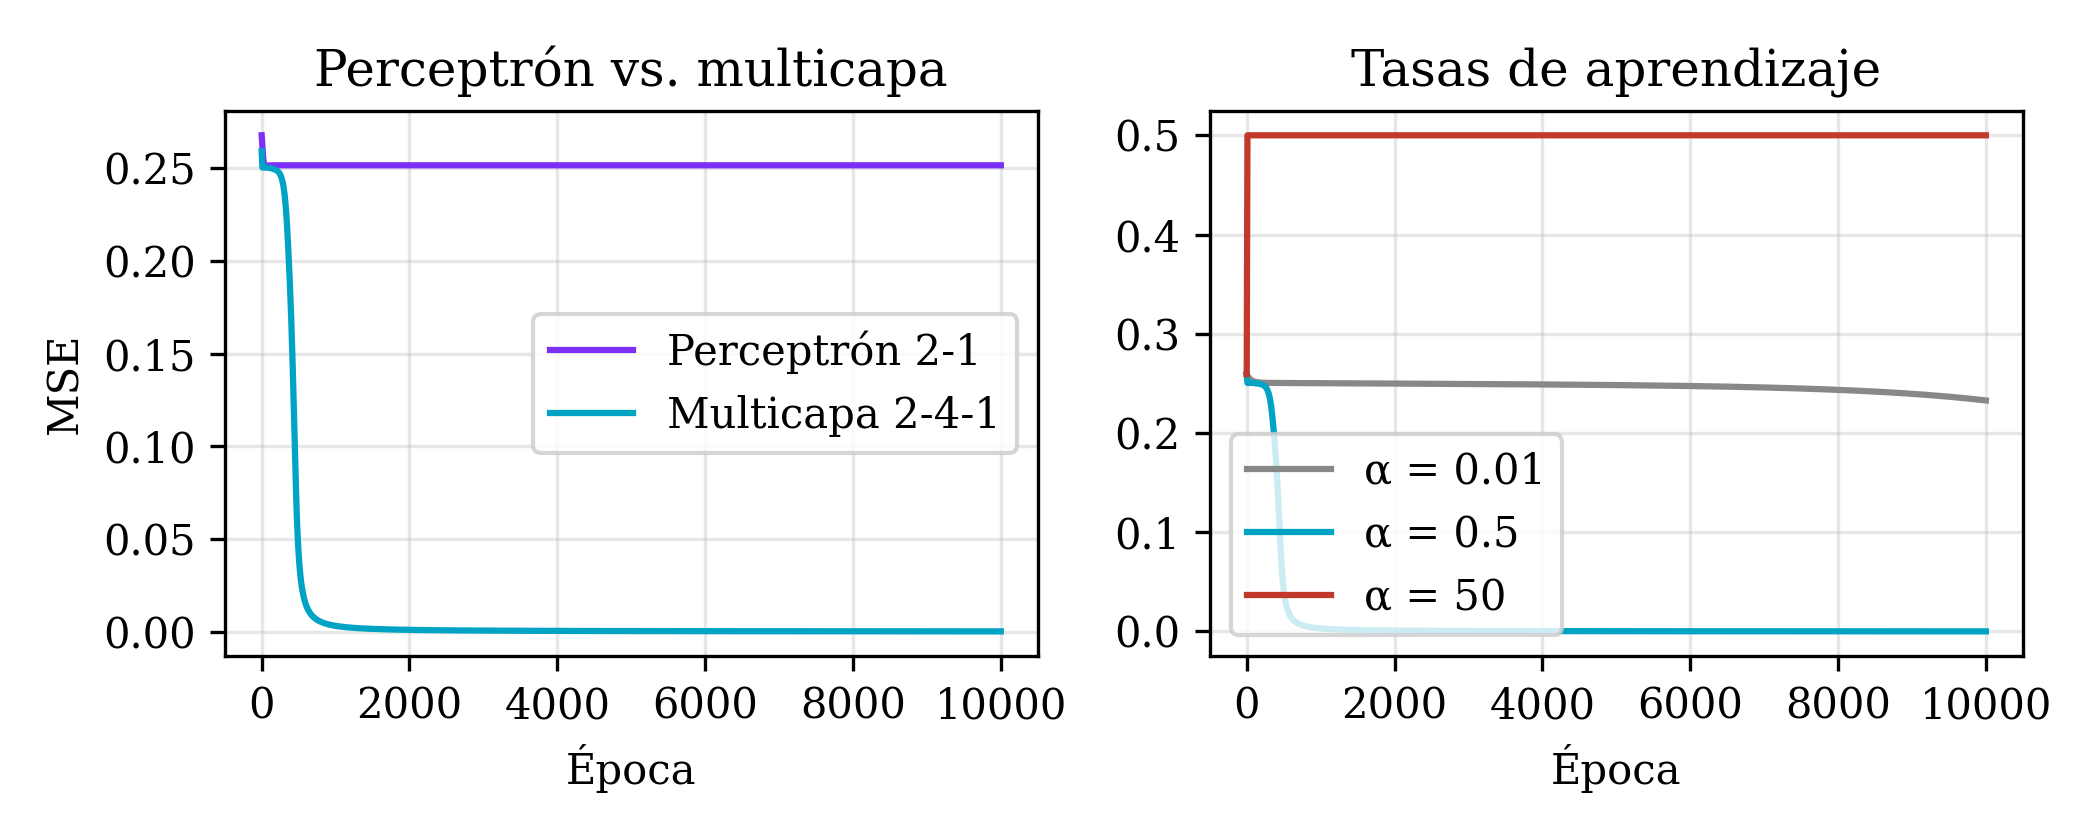
\includegraphics[width=\textwidth]{figuras/exp2_xor.png}
\par\smallskip{\footnotesize\raggedright\emph{Nota.} Izquierda: perceptrón frente a red multicapa. Derecha: tasas de aprendizaje baja, óptima y alta.\par}
\end{figure}

\subsection{Análisis}
El perceptrón no puede resolver XOR porque sus cuatro puntos no son linealmente separables: ninguna recta divide $\{(0,1),(1,0)\}$ de $\{(0,0),(1,1)\}$ \citep{minsky1969}. Su MSE se estanca cerca de $0.25$, valor que corresponde a predecir aproximadamente $0.5$ para todas las entradas. La capa oculta de la red 2-4-1 transforma el espacio de entrada en una representación donde las clases sí son separables, lo que confirma empíricamente el teorema de aproximación universal \citep{cybenko1989}.

Respecto a la tasa de aprendizaje, con $\alpha=0.01$ la red apenas avanza en \EdosEpocas{} épocas (MSE de \EdosMseBaja); con $\alpha=0.5$ converge en la época \EdosConvOptima; y con $\alpha=50$ los pasos son tan grandes que las neuronas Sigmoid se saturan, sus derivadas se anulan y el aprendizaje se detiene con MSE de \EdosMseAlta, lo que ilustra la importancia de elegir correctamente este hiperparámetro \citep{ruder2016}.

\section{Experimento 3: clasificación de vocales}\label{sec:exp3}
\subsection{Diseño del conjunto de datos}
Cada vocal se representa como una matriz binaria de $5\times5$ (Figura~\ref{fig:prototipos}), aplanada en un vector de 25 entradas. La salida usa codificación \emph{one-hot} de 5 posiciones. El conjunto de entrenamiento contiene \EtresNEnt{} muestras (los 5 prototipos y 4 variantes por vocal con un píxel invertido). El conjunto de prueba contiene \EtresNPru{} muestras distintas de las de entrenamiento: 10 variantes por vocal para cada nivel de ruido de 1 a 5 píxeles invertidos.

\begin{figure}[H]
\caption{Prototipos binarios $5\times5$ de las vocales}\label{fig:prototipos}
\centering
\includegraphics[width=0.75\textwidth]{figuras/vocales_prototipos.png}
\par\smallskip{\footnotesize\raggedright\emph{Nota.} Negro = 1, blanco = 0. Fuente: \texttt{resultados/dataset\_vocales.csv}.\par}
\end{figure}

\subsection{Resultados}
La red 25-10-5 (Sigmoid/Sigmoid, 315 parámetros) se entrenó durante \EtresEpocas{} épocas con $\alpha=\EtresAlpha$. Alcanzó en entrenamiento un MSE de \EtresMseEnt{} con exactitud de \EtresAccEnt, y en prueba un MSE de \EtresMsePru{} con exactitud de \EtresAccPru. La Tabla~\ref{tab:ruido} desglosa la exactitud por nivel de ruido y la Tabla~\ref{tab:confusion} presenta la matriz de confusión.

\begin{table}[H]
\caption{Exactitud de prueba por nivel de ruido}\label{tab:ruido}
\small
\begin{tabular}{@{}rrr@{}}
\toprule
Píxeles invertidos & Muestras & Exactitud \\
\midrule
\TablaEtresRuido
\bottomrule
\end{tabular}
\par\smallskip{\footnotesize\emph{Nota.} Fuente: \texttt{resultados/resumen.csv}.}
\end{table}

\begin{table}[H]
\caption{Matriz de confusión del conjunto de prueba}\label{tab:confusion}
\small
\begin{tabular}{@{}l ccccc@{}}
\toprule
& \multicolumn{5}{c}{Predicha} \\
\cmidrule(l){2-6}
Real & A & E & I & O & U \\
\midrule
\TablaConfusion
\bottomrule
\end{tabular}
\par\smallskip{\footnotesize\emph{Nota.} Filas: clase real; columnas: clase predicha. Fuente: \texttt{resultados/exp3\_confusion.csv}.}
\end{table}

\begin{figure}[H]
\caption{Entrenamiento y matriz de confusión del Experimento 3}\label{fig:exp3}
\centering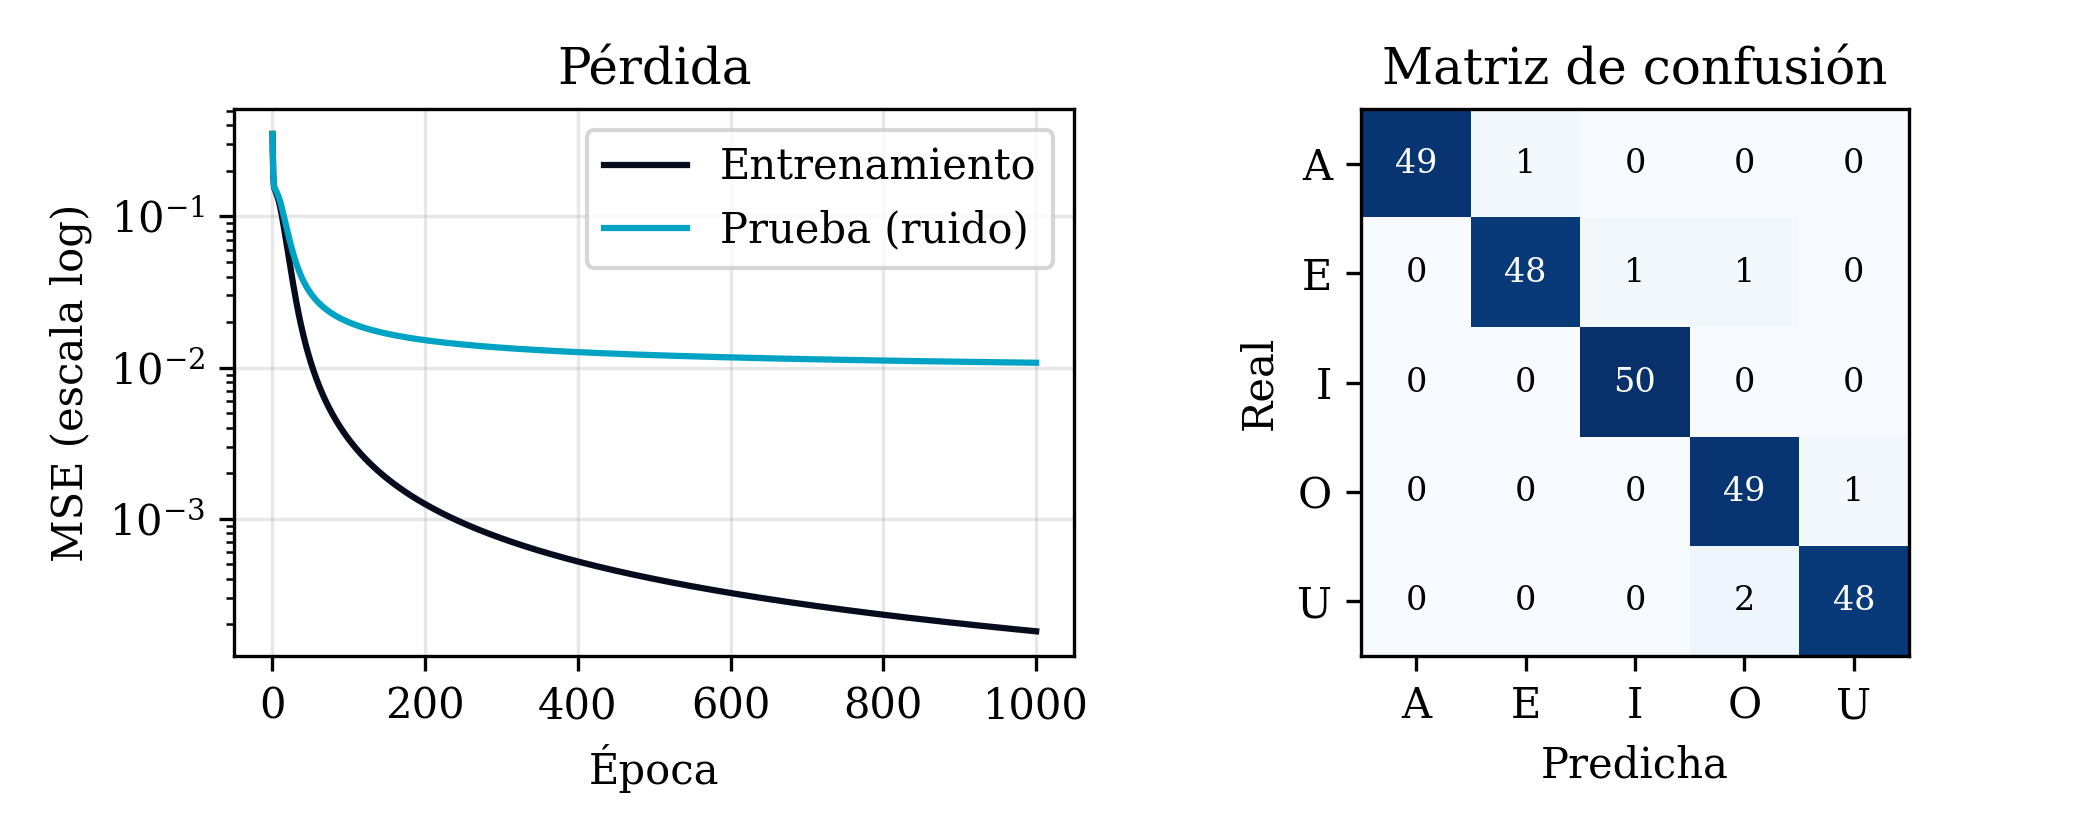
\includegraphics[width=\textwidth]{figuras/exp3_vocales.png}
\par\smallskip{\footnotesize\raggedright\emph{Nota.} Izquierda: MSE de entrenamiento y de prueba. Derecha: matriz de confusión.\par}
\end{figure}

\subsection{Análisis}
La red clasifica sin errores todas las muestras con hasta 3 píxeles invertidos (12\,\% de la imagen), aunque solo vio variantes con un píxel alterado durante el entrenamiento. Con 4 y 5 píxeles invertidos (16\,\% y 20\,\%) la exactitud desciende al 94\,\%. Los errores se concentran entre pares de vocales visualmente parecidas: O y U comparten los laterales y la base, y E comparte la columna izquierda con otras letras. Este comportamiento es coherente con la representación aprendida y muestra la capacidad de generalización del modelo frente a ruido no observado.

\section{Rendimiento y benchmarks}
Los tiempos se midieron con \texttt{std::time::Instant} sobre el binario compilado en modo \emph{release} (sistema \BenchSO, arquitectura \BenchArch), como promedio de 3 repeticiones; la inferencia se promedió sobre 100\,000 predicciones. El binario resultante ocupa \BinKiB~KiB.

\begin{table}[H]
\caption{Tiempos reales de entrenamiento e inferencia}\label{tab:bench}
\small
\begin{tabular}{@{}llrrrrr@{}}
\toprule
Experimento & Red & Parám. & Épocas & Entren. (ms) & µs/época & Inferencia (ns) \\
\midrule
\TablaBench
\bottomrule
\end{tabular}
\par\smallskip{\footnotesize\emph{Nota.} Los tiempos dependen del equipo utilizado. Fuente: \texttt{resultados/benchmarks.csv}.}
\end{table}

El costo por época se mantiene aproximadamente constante para cada arquitectura, lo que confirma la complejidad lineal $O(E\cdot N\cdot P)$ del entrenamiento (épocas $\times$ muestras $\times$ parámetros). Incluso 100\,000 épocas de XOR se completan en menos de medio segundo, lo que demuestra que no se requiere hardware especializado para estudiar estos fundamentos.

\chapter{Conclusiones}\label{cap:conclusiones}
A partir de la implementación y de los resultados experimentales reales, se presentan las conclusiones del proyecto organizadas según los objetivos planteados.

\begin{enumerate}[leftmargin=2em,itemsep=4pt]
\item \textbf{Objetivo general.} Se construyó una red neuronal multicapa funcional en Rust utilizando únicamente la biblioteca estándar, sin crates de aprendizaje automático ni de álgebra lineal, capaz de resolver problemas de regresión, de lógica no lineal y de clasificación de patrones.
\item \textbf{Álgebra lineal (OE1).} Las estructuras \texttt{Vector} y \texttt{Matrix} implementan todas las operaciones requeridas y detectan los errores de dimensión mediante \texttt{Result}, lo que evita resultados incorrectos silenciosos.
\item \textbf{Activaciones y pérdida (OE2).} Las derivadas analíticas de Sigmoid, ReLU, lineal y MSE coinciden con sus aproximaciones numéricas, lo que valida su implementación.
\item \textbf{Red y aprendizaje (OE3).} La retropropagación implementada en forma matricial reproduce fielmente las ecuaciones derivadas en el marco teórico y permite entrenar topologías arbitrarias de forma reproducible.
\item \textbf{Verificación (OE4).} Las 52 pruebas automatizadas se aprueban en su totalidad, incluida la verificación numérica de gradientes en redes de hasta tres capas.
\item \textbf{Experimentos (OE5).} La regresión $y=2x$ alcanzó un MSE de \EunoMseFin; el perceptrón de una capa se estancó en \EdosAccPer{} de exactitud en XOR mientras la red 2-4-1 logró \EdosAccMul, lo que confirma la necesidad de capas ocultas para problemas no lineales; y la clasificación de vocales obtuvo \EtresAccPru{} de exactitud sobre muestras con ruido no vistas.
\item \textbf{Rendimiento (OE6).} El binario optimizado ocupa \BinKiB~KiB y entrena cualquiera de los experimentos en fracciones de segundo, lo que demuestra que los fundamentos del aprendizaje automático pueden estudiarse con equipos convencionales.
\end{enumerate}

\chapter{Recomendaciones}\label{cap:recomendaciones}
Con base en la experiencia obtenida, se formulan las siguientes recomendaciones para trabajos futuros y para el uso educativo del proyecto.

\begin{enumerate}[leftmargin=2em,itemsep=4pt]
\item Incorporar entrenamiento por mini-lotes (\emph{mini-batch}) y optimizadores adaptativos como Momentum o Adam para acelerar la convergencia.
\item Añadir la función de pérdida de entropía cruzada con activación Softmax, más adecuada que el MSE para clasificación multiclase.
\item Ampliar el Experimento 3 a matrices de mayor resolución, a todo el alfabeto o a dígitos manuscritos, y separar un conjunto de validación.
\item Estudiar el efecto del número de neuronas ocultas y de la semilla aleatoria sobre la convergencia mediante experimentos repetidos.
\item Explorar la paralelización con los hilos de la biblioteca estándar de Rust para acelerar el entrenamiento de redes mayores.
\item Utilizar el repositorio como material didáctico en Programación 1, proponiendo a los estudiantes reproducir la prueba de escritorio y modificar los experimentos.
\item Para la versión final del documento, complementar la contextualización nacional y departamental con estadísticas oficiales verificables citadas en formato APA 7.
\end{enumerate}

\clearpage\phantomsection\addcontentsline{toc}{chapter}{Bibliografía}
{\singlespacing\begin{thebibliography}{99}

\bibitem[{American Psychological Association}(2020)]{apa2020}
American Psychological Association. (2020). \emph{Publication manual of the American Psychological Association} (7th ed.). \url{https://doi.org/10.1037/0000165-000}

\bibitem[{Asamblea Legislativa Plurinacional de Bolivia}(2011)]{bolivia2011}
Asamblea Legislativa Plurinacional de Bolivia. (2011). \emph{Ley N.º 164: Ley General de Telecomunicaciones, Tecnologías de Información y Comunicación}. Gaceta Oficial del Estado Plurinacional de Bolivia.

\bibitem[{Baydin et~al.}(2018)]{baydin2018}
Baydin, A. G., Pearlmutter, B. A., Radul, A. A., \& Siskind, J. M. (2018). Automatic differentiation in machine learning: A survey. \emph{Journal of Machine Learning Research}, \emph{18}(153), 1–43. \url{https://jmlr.org/papers/v18/17-468.html}

\bibitem[{Bishop}(2006)]{bishop2006}
Bishop, C. M. (2006). \emph{Pattern recognition and machine learning}. Springer.

\bibitem[{Blandy et~al.}(2021)]{blandy2021}
Blandy, J., Orendorff, J., \& Tindall, L. F. S. (2021). \emph{Programming Rust: Fast, safe systems development} (2nd ed.). O'Reilly Media.

\bibitem[{Bottou}(2010)]{bottou2010}
Bottou, L. (2010). Large-scale machine learning with stochastic gradient descent. En \emph{Proceedings of COMPSTAT'2010} (pp.~177–186). Physica-Verlag. \url{https://doi.org/10.1007/978-3-7908-2604-3_16}

\bibitem[{Cybenko}(1989)]{cybenko1989}
Cybenko, G. (1989). Approximation by superpositions of a sigmoidal function. \emph{Mathematics of Control, Signals and Systems}, \emph{2}(4), 303–314. \url{https://doi.org/10.1007/BF02551274}

\bibitem[{Deisenroth et~al.}(2020)]{deisenroth2020}
Deisenroth, M. P., Faisal, A. A., \& Ong, C. S. (2020). \emph{Mathematics for machine learning}. Cambridge University Press. \url{https://doi.org/10.1017/9781108679930}

\bibitem[{Glorot y Bengio}(2010)]{glorot2010}
Glorot, X., \& Bengio, Y. (2010). Understanding the difficulty of training deep feedforward neural networks. En \emph{Proceedings of the Thirteenth International Conference on Artificial Intelligence and Statistics} (Vol.~9, pp.~249–256). PMLR. \url{https://proceedings.mlr.press/v9/glorot10a.html}

\bibitem[{Goodfellow et~al.}(2016)]{goodfellow2016}
Goodfellow, I., Bengio, Y., \& Courville, A. (2016). \emph{Deep learning}. MIT Press. \url{https://www.deeplearningbook.org/}

\bibitem[{Haykin}(2009)]{haykin2009}
Haykin, S. (2009). \emph{Neural networks and learning machines} (3rd ed.). Pearson Education.

\bibitem[{He et~al.}(2015)]{he2015}
He, K., Zhang, X., Ren, S., \& Sun, J. (2015). Delving deep into rectifiers: Surpassing human-level performance on ImageNet classification. En \emph{Proceedings of the IEEE International Conference on Computer Vision} (pp.~1026–1034). IEEE. \url{https://doi.org/10.1109/ICCV.2015.123}

\bibitem[{Hernández Sampieri y Mendoza Torres}(2018)]{hernandez2018}
Hernández Sampieri, R., \& Mendoza Torres, C. P. (2018). \emph{Metodología de la investigación: Las rutas cuantitativa, cualitativa y mixta}. McGraw-Hill Interamericana.

\bibitem[{Hornik et~al.}(1989)]{hornik1989}
Hornik, K., Stinchcombe, M., \& White, H. (1989). Multilayer feedforward networks are universal approximators. \emph{Neural Networks}, \emph{2}(5), 359–366. \url{https://doi.org/10.1016/0893-6080(89)90020-8}

\bibitem[{Jung et~al.}(2018)]{jung2018}
Jung, R., Jourdan, J.-H., Krebbers, R., \& Dreyer, D. (2018). RustBelt: Securing the foundations of the Rust programming language. \emph{Proceedings of the ACM on Programming Languages}, \emph{2}(POPL), 66:1–66:34. \url{https://doi.org/10.1145/3158154}

\bibitem[{Klabnik y Nichols}(2023)]{klabnik2023}
Klabnik, S., \& Nichols, C. (2023). \emph{The Rust programming language} (2nd ed.). No Starch Press. \url{https://doc.rust-lang.org/book/}

\bibitem[{LeCun et~al.}(1998)]{lecun1998}
LeCun, Y., Bottou, L., Orr, G. B., \& Müller, K.-R. (1998). Efficient BackProp. En G. B. Orr y K.-R. Müller (Eds.), \emph{Neural networks: Tricks of the trade} (pp.~9–50). Springer. \url{https://doi.org/10.1007/3-540-49430-8_2}

\bibitem[{LeCun et~al.}(2015)]{lecun2015}
LeCun, Y., Bengio, Y., \& Hinton, G. (2015). Deep learning. \emph{Nature}, \emph{521}(7553), 436–444. \url{https://doi.org/10.1038/nature14539}

\bibitem[{Maslej et~al.}(2024)]{maslej2024}
Maslej, N., Fattorini, L., Perrault, R., Parli, V., Reuel, A., Brynjolfsson, E., Etchemendy, J., Ligett, K., Lyons, T., Manyika, J., Niebles, J. C., Shoham, Y., Wald, R., \& Clark, J. (2024). \emph{The AI Index 2024 annual report}. AI Index Steering Committee, Institute for Human-Centered AI, Stanford University. \url{https://aiindex.stanford.edu/report/}

\bibitem[{Matsakis y Klock}(2014)]{matsakis2014}
Matsakis, N. D., \& Klock, F. S., II. (2014). The Rust language. \emph{ACM SIGAda Ada Letters}, \emph{34}(3), 103–104. \url{https://doi.org/10.1145/2692956.2663188}

\bibitem[{McCulloch y Pitts}(1943)]{mcculloch1943}
McCulloch, W. S., \& Pitts, W. (1943). A logical calculus of the ideas immanent in nervous activity. \emph{The Bulletin of Mathematical Biophysics}, \emph{5}(4), 115–133. \url{https://doi.org/10.1007/BF02478259}

\bibitem[{Minsky y Papert}(1969)]{minsky1969}
Minsky, M., \& Papert, S. (1969). \emph{Perceptrons: An introduction to computational geometry}. MIT Press.

\bibitem[{Nielsen}(2015)]{nielsen2015}
Nielsen, M. A. (2015). \emph{Neural networks and deep learning}. Determination Press. \url{http://neuralnetworksanddeeplearning.com/}

\bibitem[{Rosenblatt}(1958)]{rosenblatt1958}
Rosenblatt, F. (1958). The perceptron: A probabilistic model for information storage and organization in the brain. \emph{Psychological Review}, \emph{65}(6), 386–408. \url{https://doi.org/10.1037/h0042519}

\bibitem[{Ruder}(2016)]{ruder2016}
Ruder, S. (2016). \emph{An overview of gradient descent optimization algorithms}. arXiv. \url{https://doi.org/10.48550/arXiv.1609.04747}

\bibitem[{Rumelhart et~al.}(1986)]{rumelhart1986}
Rumelhart, D. E., Hinton, G. E., \& Williams, R. J. (1986). Learning representations by back-propagating errors. \emph{Nature}, \emph{323}(6088), 533–536. \url{https://doi.org/10.1038/323533a0}

\bibitem[{Russell y Norvig}(2021)]{russell2021}
Russell, S., \& Norvig, P. (2021). \emph{Artificial intelligence: A modern approach} (4th ed.). Pearson.

\bibitem[{Stack Overflow}(2024)]{stackoverflow2024}
Stack Overflow. (2024). \emph{2024 Stack Overflow developer survey}. \url{https://survey.stackoverflow.co/2024/}

\bibitem[{Strang}(2016)]{strang2016}
Strang, G. (2016). \emph{Introduction to linear algebra} (5th ed.). Wellesley-Cambridge Press.

\bibitem[{UNESCO}(2022)]{unesco2022}
UNESCO. (2022). \emph{Recommendation on the ethics of artificial intelligence}. United Nations Educational, Scientific and Cultural Organization. \url{https://unesdoc.unesco.org/ark:/48223/pf0000381137}

\end{thebibliography}
}
\appendix
\renewcommand{\chaptername}{Anexo}
\titleformat{\chapter}[display]{\normalfont\bfseries\color{marino}\centering}{\large ANEXO \thechapter}{4pt}{\LARGE}

\chapter{Resumen de pruebas \texttt{cargo test}}\label{anx:tests}
El siguiente listado corresponde a la salida real de \texttt{cargo test} sobre el código del repositorio. Las 52 pruebas se aprueban sin fallos.
{\singlespacing\lstinputlisting[language={},basicstyle=\ttfamily\scriptsize,numbers=none,caption={Salida de \texttt{cargo test}},label=cod:tests]{generado/cargo_test.txt}}

\chapter{Extracto de código fuente en Rust}\label{anx:codigo}
Se presentan extractos representativos del código fuente. El código completo, documentado con comentarios \texttt{///} en español, está disponible en el repositorio del proyecto: \url{\Repositorio}.

\lstinputlisting[caption={Función Sigmoid y su derivada (\texttt{src/nn/activation.rs})},label=cod:sigmoid]{generado/codigo/sigmoid.rs}
\lstinputlisting[caption={Error cuadrático medio y su gradiente (\texttt{src/nn/loss.rs})},label=cod:mse]{generado/codigo/mse.rs}
\lstinputlisting[caption={Propagación hacia adelante de una capa (\texttt{src/nn/layer.rs})},label=cod:forward]{generado/codigo/layer_forward.rs}

\section*{Manual breve de uso con Cargo}
\begin{lstlisting}[language={},numbers=none,caption={Comandos de compilación y ejecución},label=cod:manual]
cargo test                         # 52 pruebas unitarias
cargo run --release -- --all       # experimentos + CSV en resultados/
cargo run --release -- --exp2      # solo XOR (también --exp1, --exp3)
cargo run --release -- --bench     # benchmarks
cargo run --release -- --all --export otra_carpeta --seed 7
\end{lstlisting}

\chapter{Carta de Compromiso}\label{anx:carta}
\begin{center}
\includegraphics[width=0.82\textwidth,height=0.8\textheight,keepaspectratio]{\CartaCompromiso}
\end{center}

\end{document}
